\chapter{Desenvolvimento do sistema} 
\label{cap4_Desenvolvimento_do_sistema} 
\section{Estrutura Mecânica}

Este capítulo apresenta os aspectos relacionados ao desenvolvimento da estrutura mecânica do sistema automatizado, estabelecendo uma base consistente para a construção, operação e validação do protótipo proposto.

Inicialmente, foi projetada uma estrutura mecânica simplificada, com a finalidade de sustentar adequadamente os componentes do sistema e garantir estabilidade durante a operação. A base estrutural foi confeccionada em madeira, material escolhido em razão de sua facilidade de manuseio, baixo custo e resistência mecânica compatível com aplicações em prototipagem.

Sobre essa base, foi desenvolvido um suporte específico para o acoplamento do painel fotovoltaico, fabricado por meio de impressão 3D. A utilização dessa tecnologia proporcionou maior precisão dimensional, flexibilidade no projeto e facilidade na adaptação dos componentes, possibilitando um ajuste geométrico mais adequado entre o painel e o sistema de acionamento.

No suporte projetado, foi fixado um motor, acoplado a um sistema de engrenagens responsável pela transmissão do movimento rotacional ao painel fotovoltaico. Esse conjunto mecânico permite o ajuste angular controlado do painel ao longo do dia, possibilitando o acompanhamento da trajetória aparente do Sol.

As Figuras~\ref{fig:engrenagem1} e~\ref{fig:engrenagem2} apresentam o suporte e as engrenagens desenvolvidas por meio de impressão 3D, utilizadas no sistema de transmissão mecânica do protótipo.
\begin{figure}[H]
    \centering
    \begin{minipage}{0.45\linewidth}
        \centering
        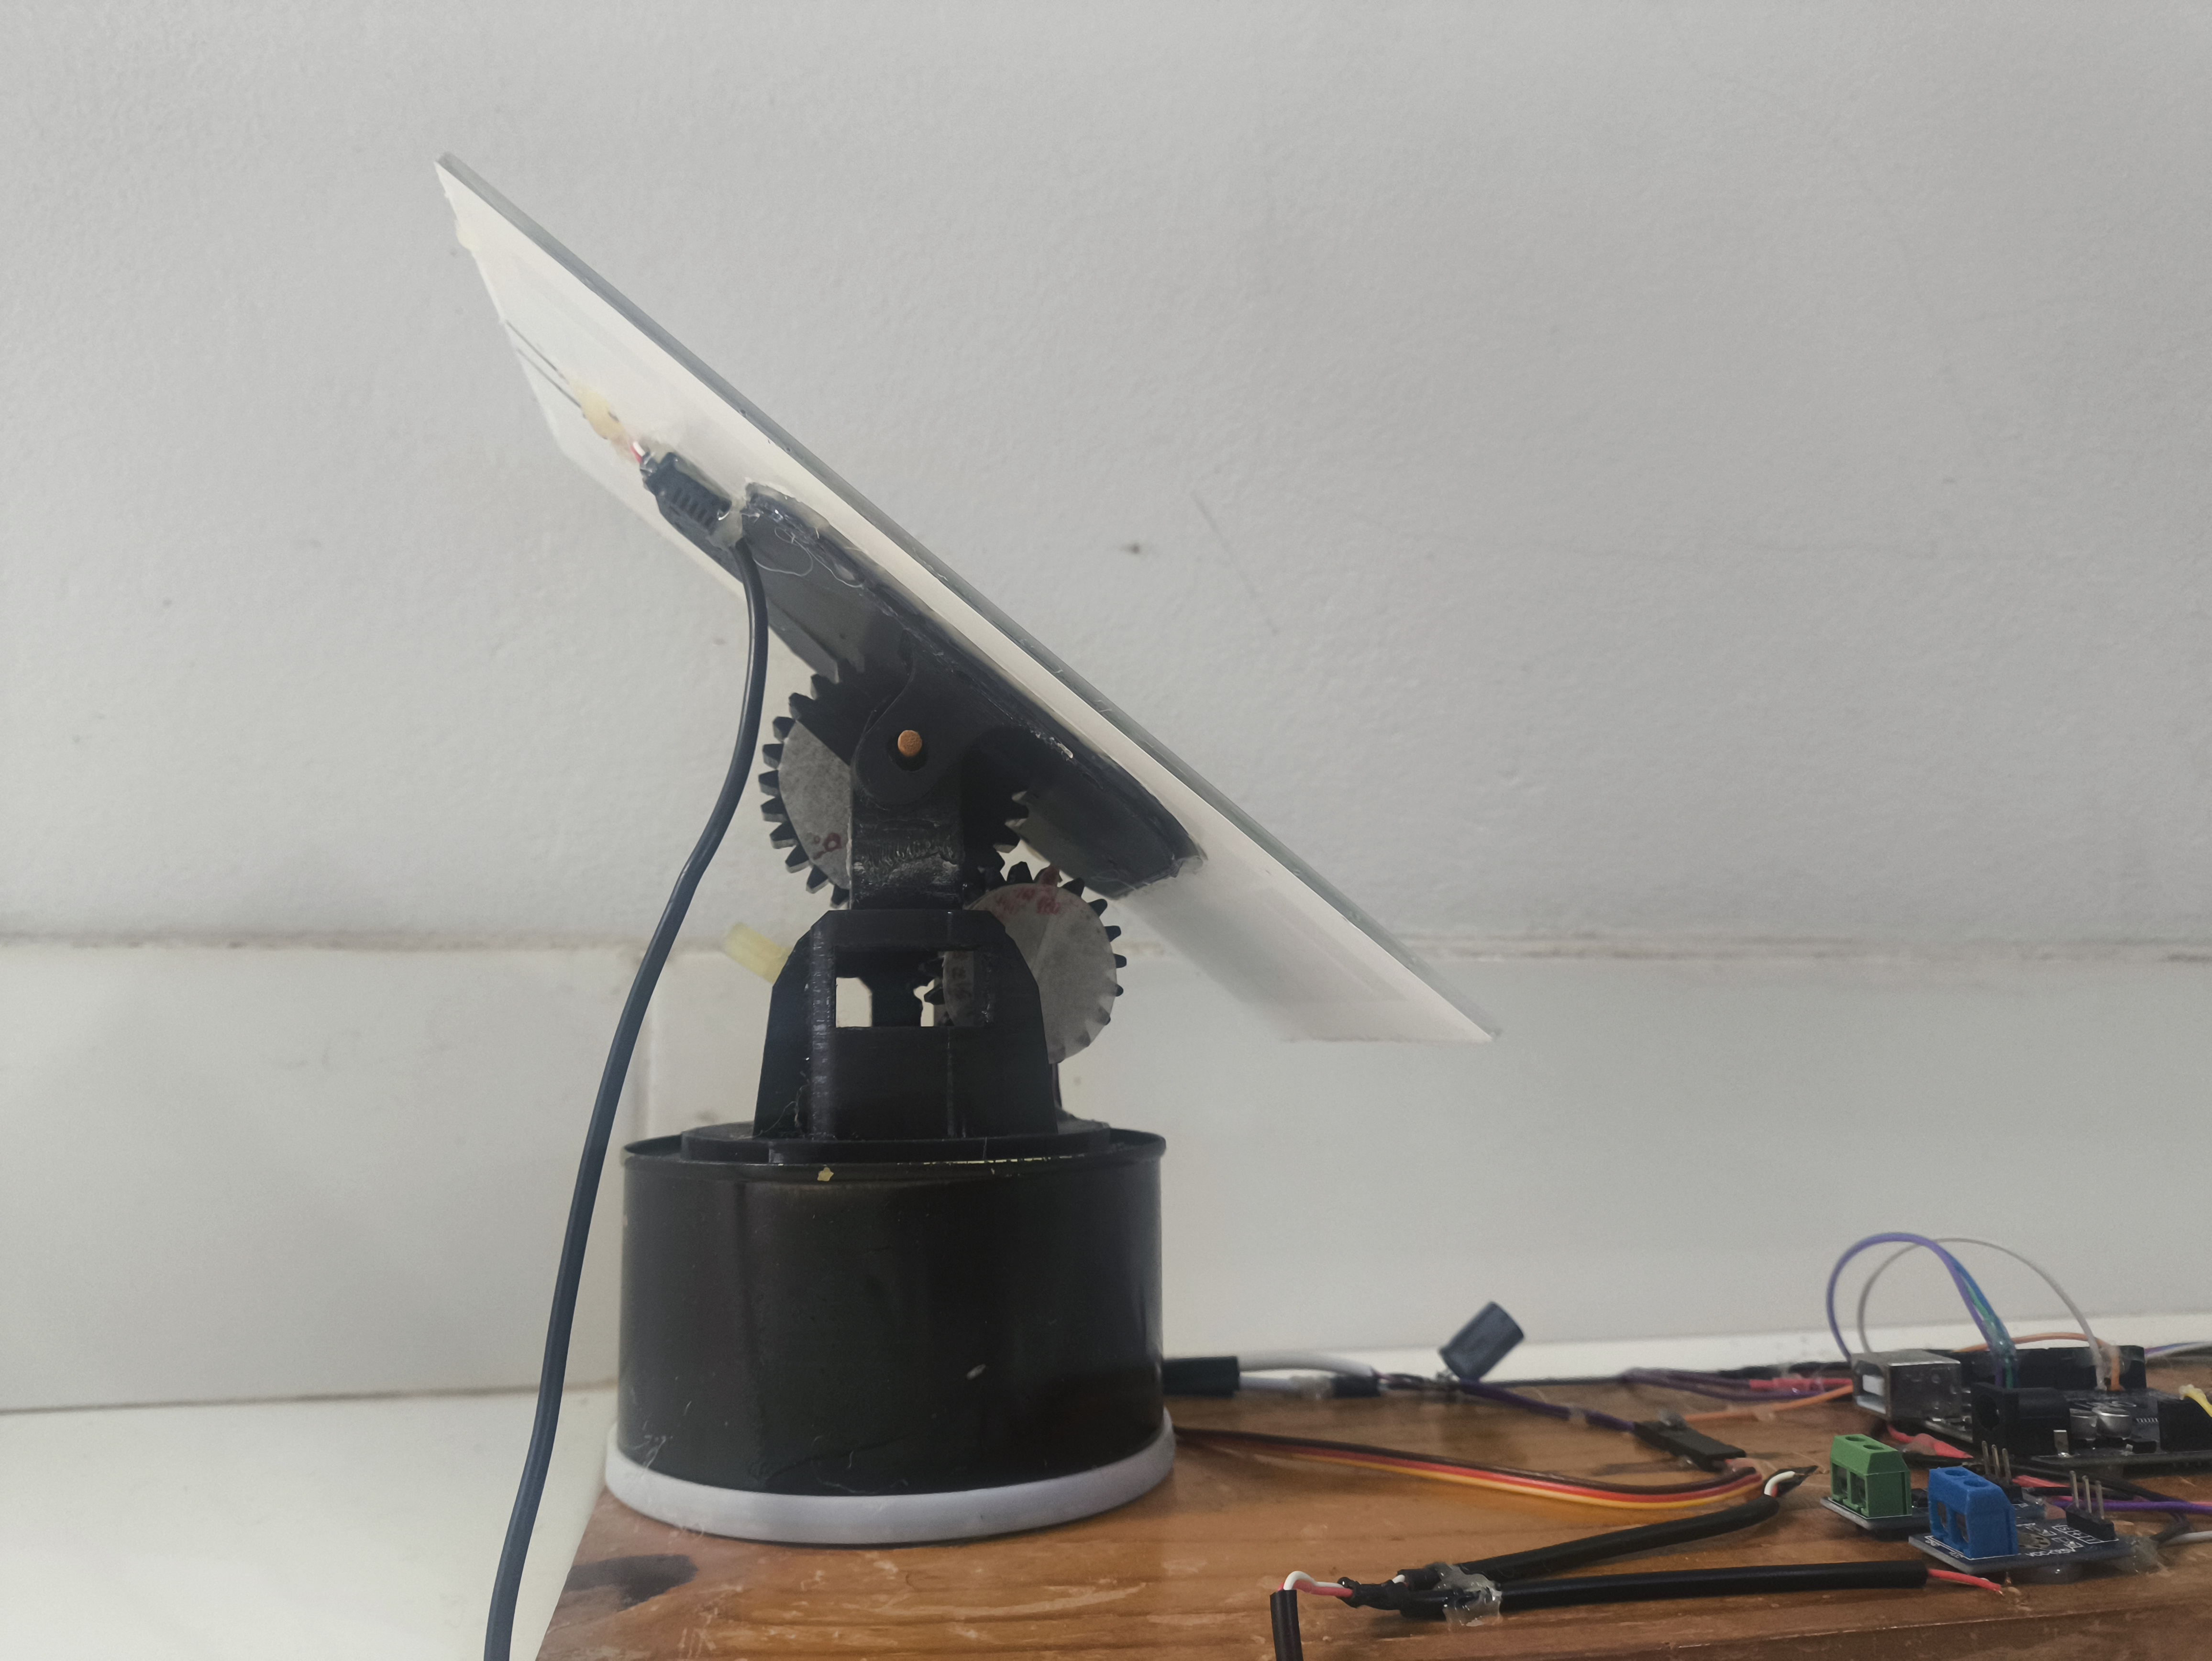
\includegraphics[width=\linewidth]{Figuras/engrenagem1.jpg}
        \caption{Suporte e Engrenagem em 3D}
        \label{fig:engrenagem1}
        \legend{Fonte: Autor (2026).}
    \end{minipage}
    \hfill
    \begin{minipage}{0.45\linewidth}
        \centering
        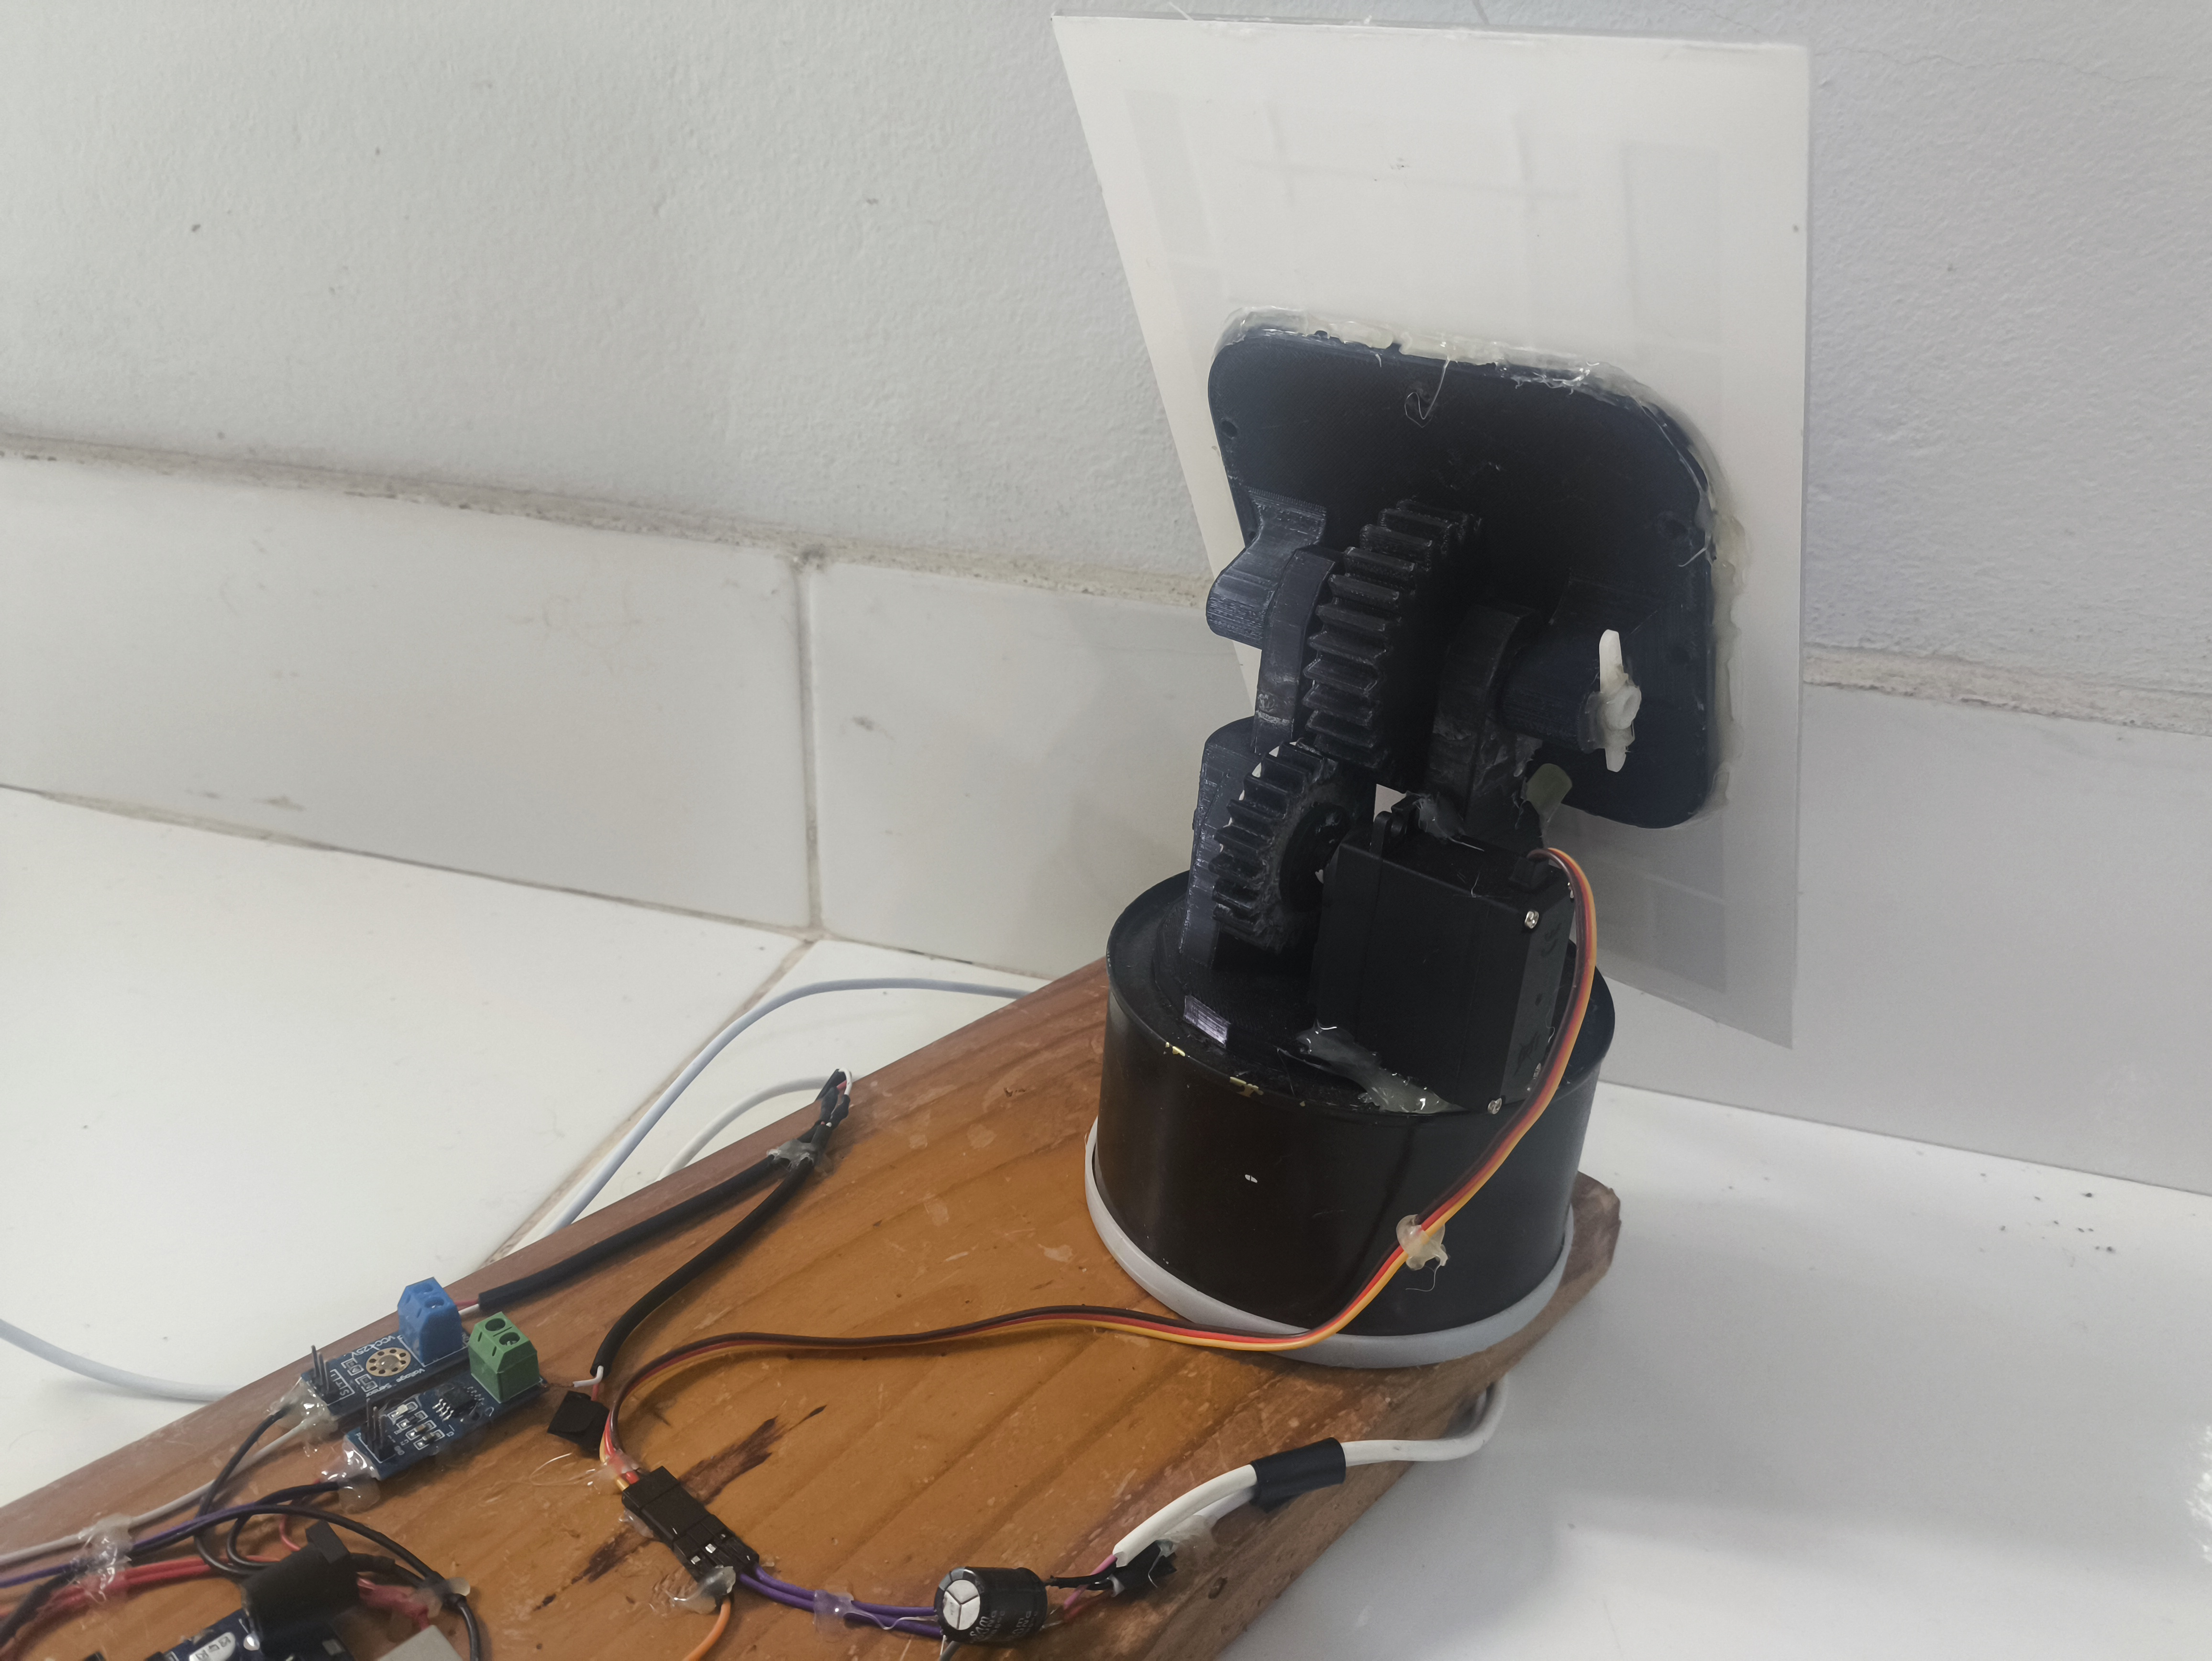
\includegraphics[width=\linewidth]{Figuras/engrenagem2.jpg}
        \caption{Detalhamento da engrenagem}
        \label{fig:engrenagem2}
        \legend{Fonte: Autor (2026).}
    \end{minipage}
\end{figure}

A base também foi utilizada para a fixação dos componentes eletrônicos do sistema de controle, incluindo o microcontrolador, sensores e módulos auxiliares, garantindo organização estrutural, redução de interferências e maior confiabilidade no funcionamento do sistema.

A Figura~\ref{fig:prototipo_montado} apresenta o protótipo do sistema desenvolvido, evidenciando a estrutura mecânica proposta e a disposição dos componentes descritos.
\begin{figure}[H]
    \centering
    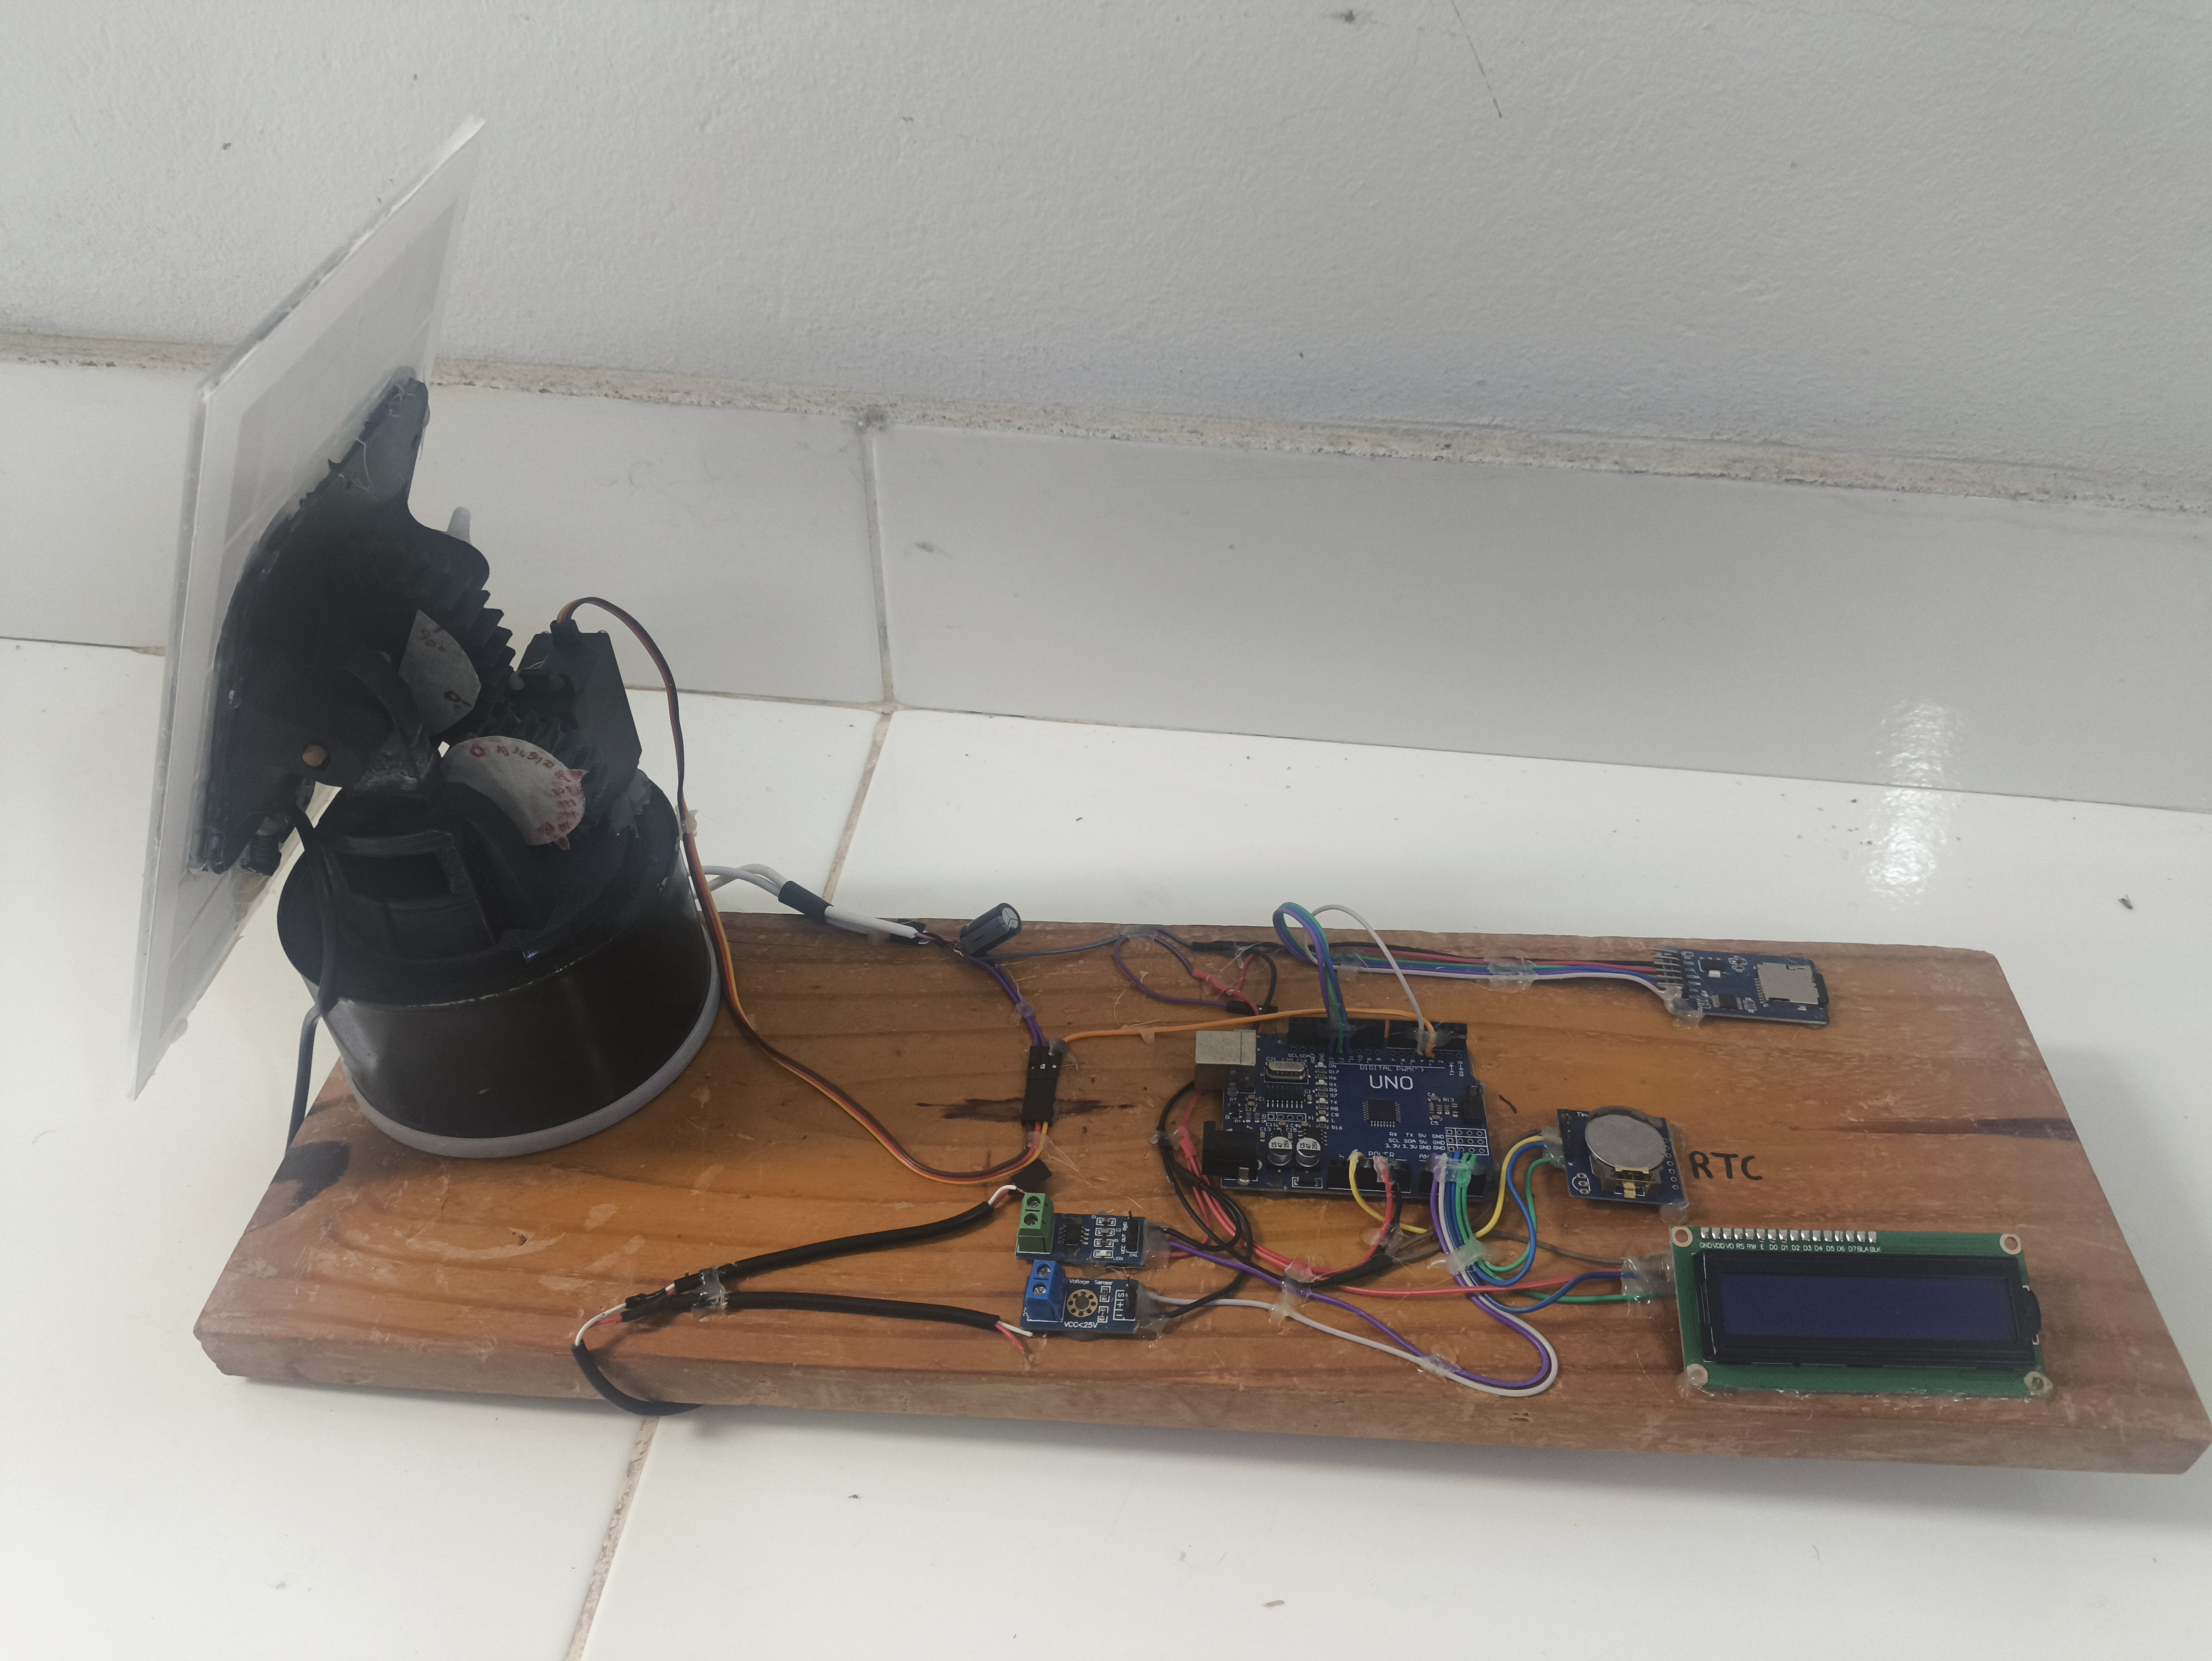
\includegraphics[width=0.6\linewidth]{Figuras/prototipo_montado.jpg}
    \caption{Protótipo do sistema automatizado desenvolvido}
    \label{fig:prototipo_montado}
    \legend{Fonte: Autor (2026).}
\end{figure}

O movimento realizado pelo servo motor corresponde à rotação do sistema em torno de um único eixo, estando diretamente associado ao deslocamento aparente do Sol no céu, no sentido Leste–Oeste. Esse movimento constitui o princípio de funcionamento do sistema automatizado de eixo único desenvolvido neste trabalho, permitindo maximizar a incidência de radiação solar sobre o painel fotovoltaico ao longo do dia.

Durante o desenvolvimento da estrutura mecânica, foram priorizados critérios como simplicidade construtiva, baixo custo, robustez e facilidade de manutenção, considerados essenciais para a viabilidade prática da proposta. Além disso, buscou-se minimizar folgas mecânicas e desalinhamentos que pudessem comprometer a precisão do sistema.

Posteriormente, foi implementada uma estrutura de isolamento ao redor do protótipo, com o objetivo de proteger os componentes eletrônicos contra intempéries, como chuva e umidade, bem como contra a incidência direta de radiação solar e possíveis interferências externas, como a presença de aves. Tais condições poderiam ocasionar danos aos componentes eletrônicos e comprometer a confiabilidade da coleta de dados. A solução adotada é apresentada na Figura~\ref{fig:protecao_prototipo}.

\begin{figure}[H]
    \centering
    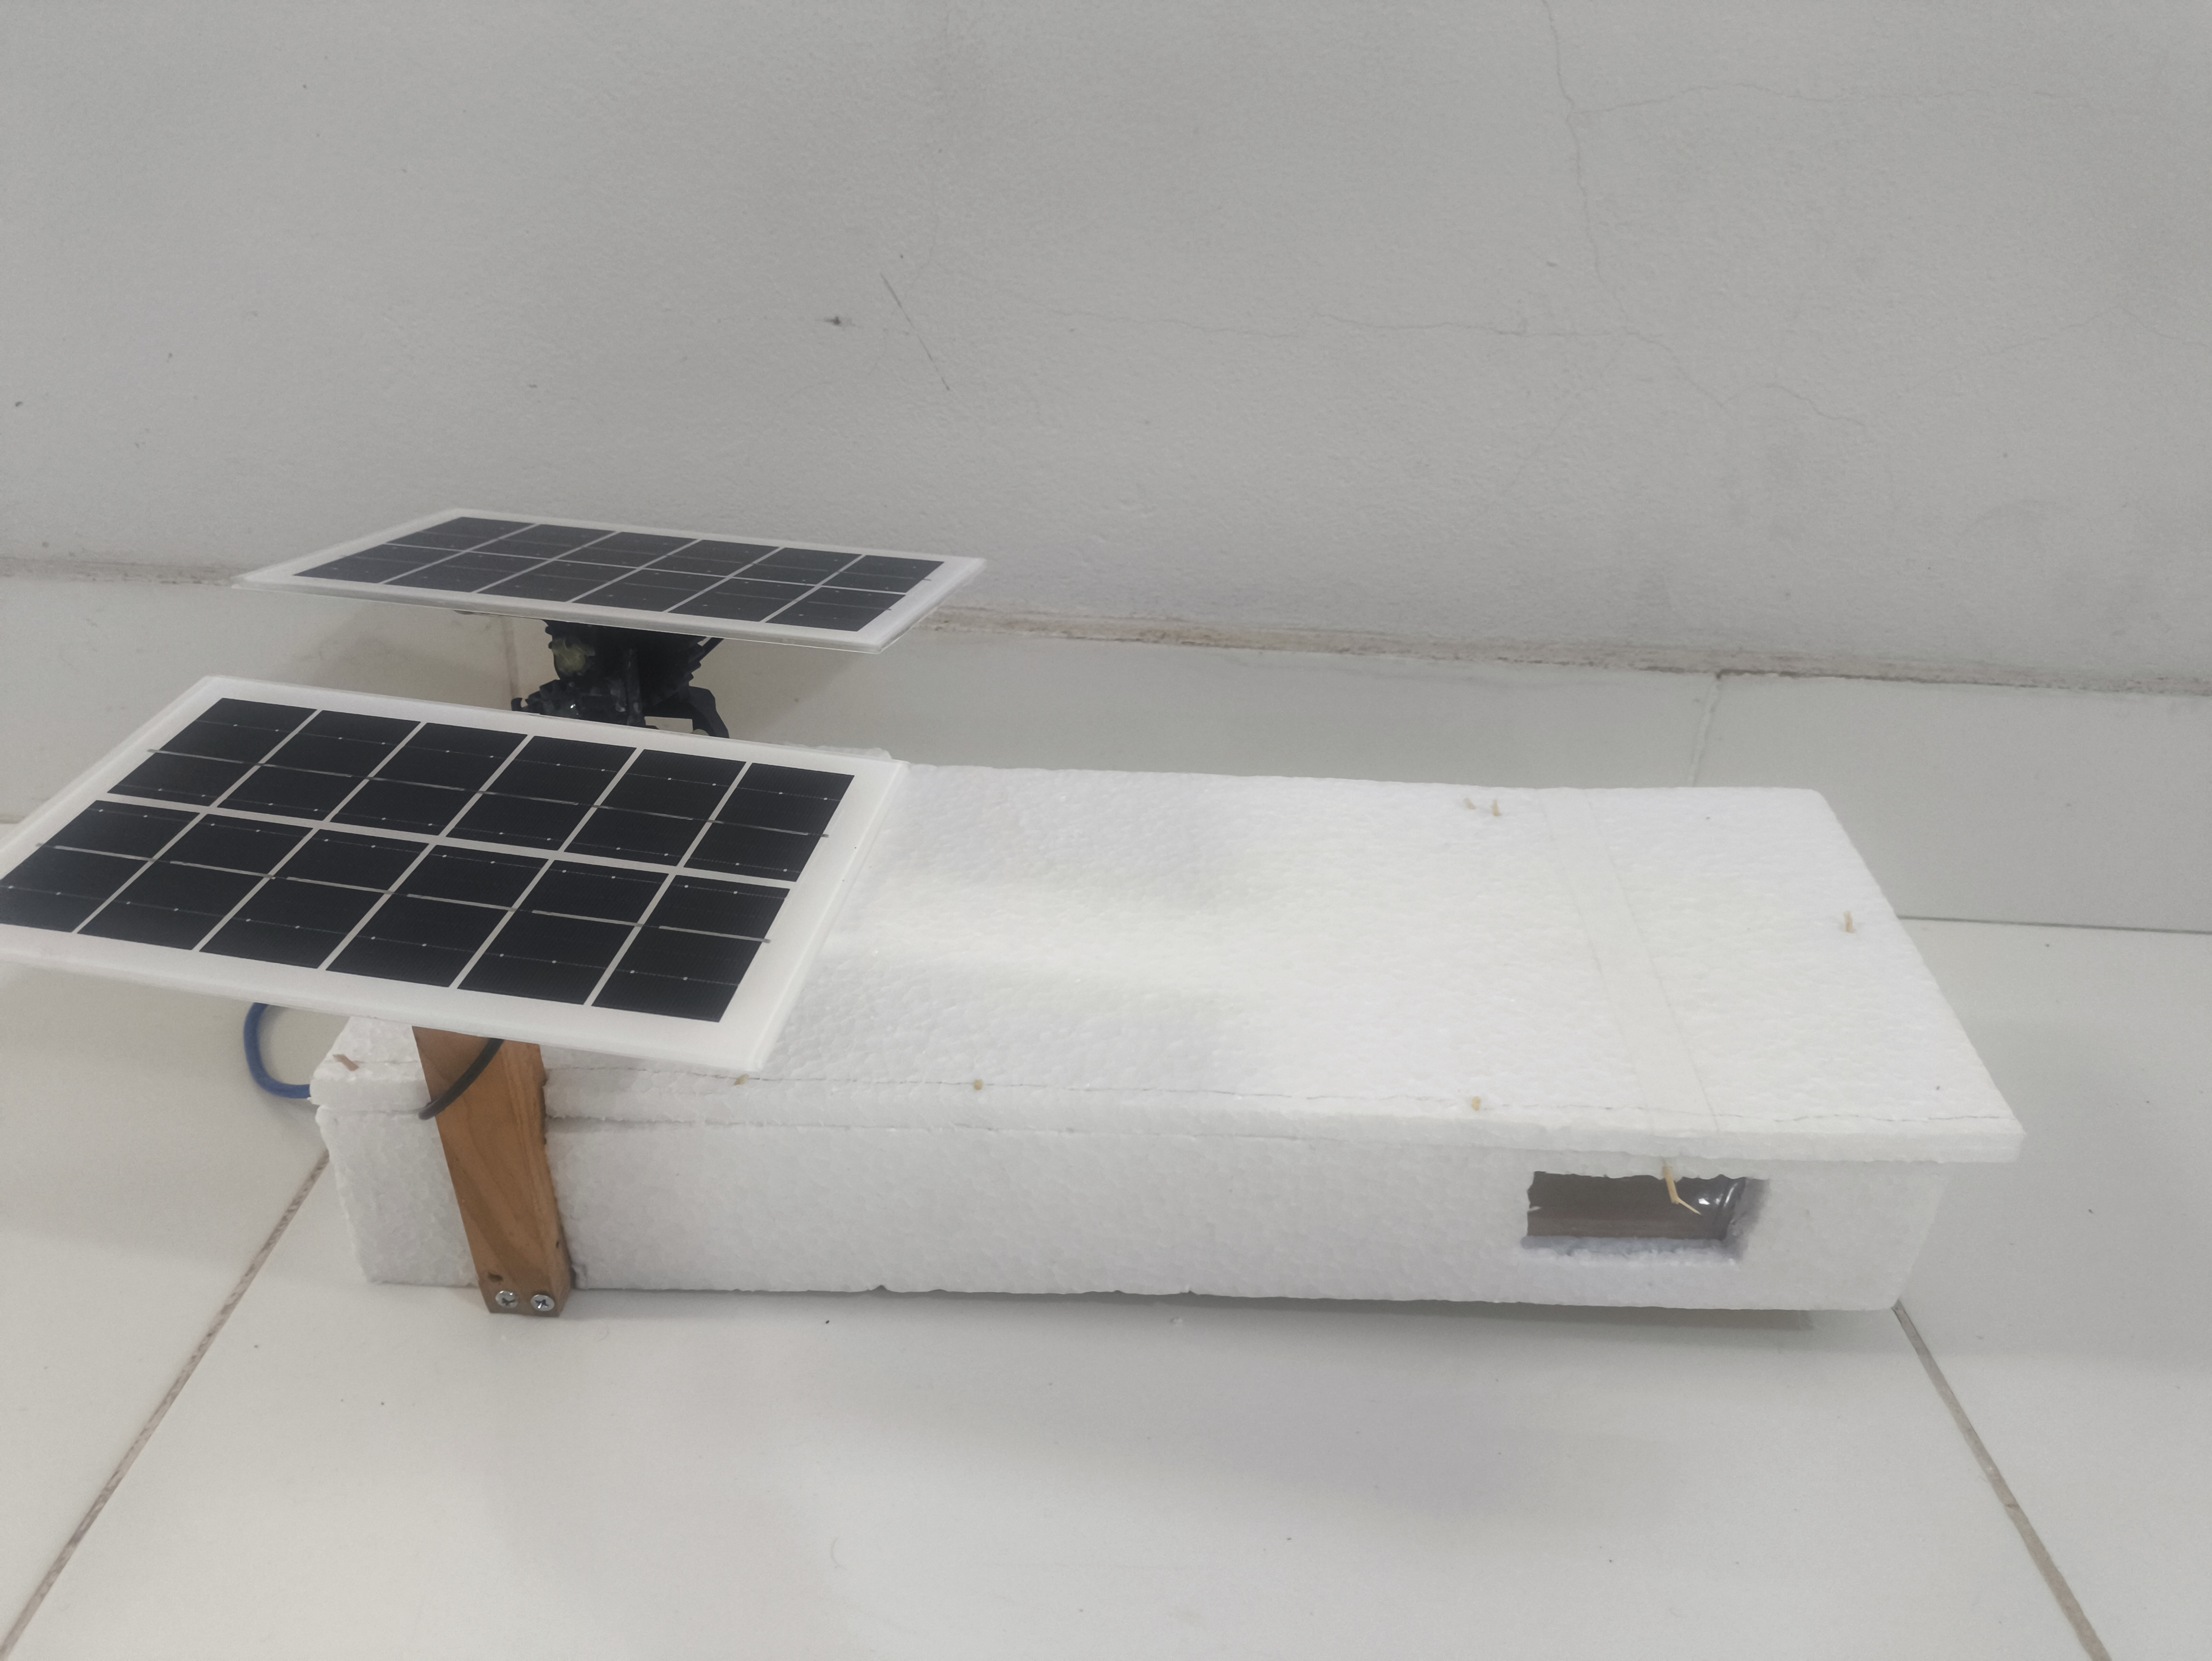
\includegraphics[width=0.7\linewidth]{Figuras/proteçao_prototipo.jpg}
    \caption{Estrutura de proteção do protótipo}
    \legend{Fonte: Autor (2026)}
    \label{fig:protecao_prototipo}
\end{figure}
\vspace{-0.4cm}
A seguir, serão apresentados os componentes utilizados na construção do sistema.
\vspace{-0.4cm}

\subsection{Arduino Uno}


Para atuar como controlador do sistema, foi selecionado o Arduino Uno, em razão de sua ampla utilização, robustez e extensa documentação disponível, fatores que facilitam sua aplicação em projetos acadêmicos e de prototipagem. O Arduino Uno é uma placa de microcontrolador baseada no ATmega328P, que possui 14 pinos de entrada e saída digitais, dos quais 6 podem ser utilizados como saídas Pulse Width Modulation (PWM), além de entradas analógicas que permitem a leitura de sinais provenientes de sensores \cite{arduino2023}.
conforme apresentado na Figura \ref{fig:arduino_uno}.
\begin{figure}[H]
    \centering
    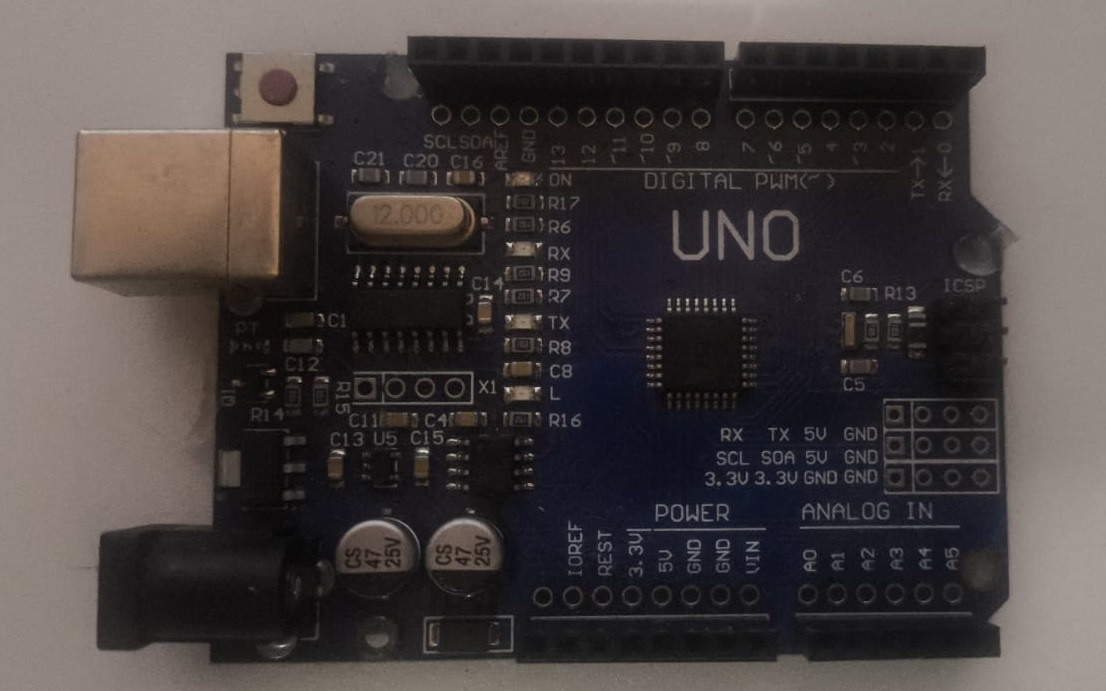
\includegraphics[width=0.6\textwidth]{Figuras/Placa Arduino Uno.jpeg}
    \caption{Placa Arduino Uno}
    \caption*{Fonte: Autor (2026).}
    \label{fig:arduino_uno}
\end{figure}


A placa reúne os recursos necessários para o desenvolvimento de sistemas embarcados, oferecendo suporte adequado à integração entre sensores, atuadores e módulos de comunicação. Sua arquitetura simplificada, aliada ao ambiente de desenvolvimento integrado, permite a programação em linguagem baseada em C e C++, contribuindo para a implementação eficiente da lógica de controle do sistema.

No contexto deste trabalho, o Arduino Uno desempenha papel central no processamento das informações, sendo responsável pela aquisição dos dados provenientes dos sensores utilizados. A partir desses dados, o microcontrolador executa rotinas programadas que determinam o posicionamento angular adequado do painel fotovoltaico ao longo do dia, com base na trajetória aparente do Sol.

Adicionalmente, o Arduino realiza o envio de sinais de controle ao atuador responsável pelo ajuste da inclinação do painel, garantindo o acompanhamento contínuo da posição solar. Paralelamente, o sistema executa o gerenciamento e o registro dos dados coletados, armazenando informações como tensão, corrente, potência e posição angular, o que possibilita análises posteriores e a validação experimental do desempenho do sistema.

Dessa forma, o Arduino Uno atua como a unidade central de processamento de um sistema embarcado, integrando as etapas de aquisição, processamento, controle e armazenamento de dados em tempo real. Tal aplicação evidencia a utilização de conceitos fundamentais de programação, automação e integração entre hardware e software, essenciais para o desenvolvimento de soluções tecnológicas eficientes e de baixo custo.

\subsection{Servo Motor}

O servo motor utilizado no desenvolvimento do protótipo foi o modelo MG996R, selecionado em razão de suas características de desempenho, como elevado torque, boa precisão de posicionamento e robustez mecânica, aspectos considerados fundamentais para aplicações que exigem controle angular confiável, conforme apresentado na Figura~\ref{fig:servo_mg996r}.

\begin{figure}[H]
    \centering
    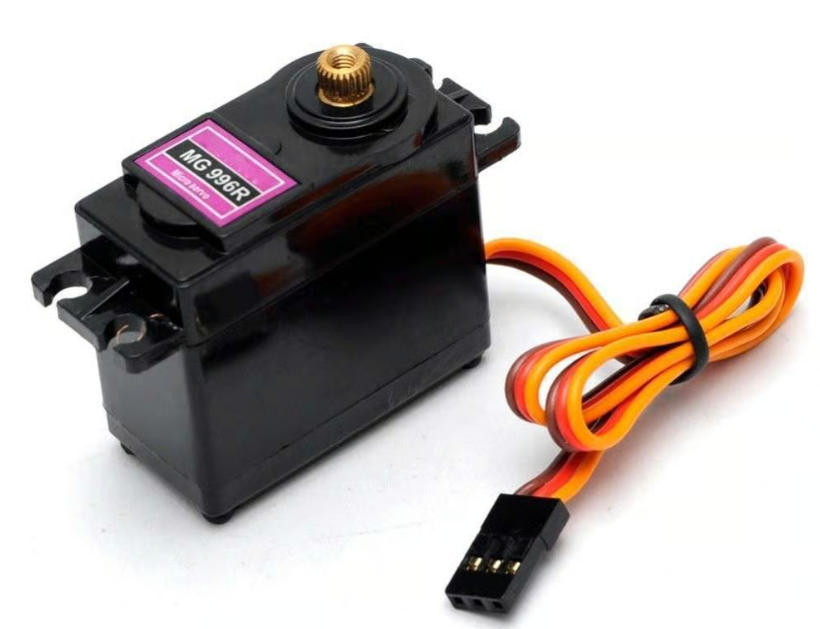
\includegraphics[width=0.6\textwidth]{Figuras/servo motor.png}
    \caption{Servo motor MG996R}
    \caption*{Fonte: Fonte: Adaptado de Eletrônica Castro (2026)}
    \label{fig:servo_mg996r}
\end{figure}

Esse atuador apresenta uma faixa de rotação aproximada de 0° a 180°, sendo constituído por um sistema interno de controle que integra um motor de corrente contínua (DC), um conjunto de engrenagens, um potenciômetro de realimentação e um circuito eletrônico de controle. Esse conjunto permite o posicionamento preciso do eixo em função do sinal de controle recebido, garantindo estabilidade e repetibilidade nos movimentos. Tais características justificam sua ampla aplicação em projetos de robótica, automação e sistemas embarcados \cite{towerpro2019}.

No contexto deste trabalho, o servo motor desempenha a função de elemento de acionamento do sistema, sendo responsável pela movimentação do painel fotovoltaico. O controle do posicionamento angular é realizado pelo Arduino por meio de sinais PWM, nos quais a largura do pulso está diretamente relacionada ao ângulo desejado, permitindo o posicionamento preciso do servomotor \cite{arduino_servo}. Dessa forma, o sistema ajusta continuamente a inclinação do painel com base nas informações de tempo fornecidas pelo sistema, possibilitando o acompanhamento da trajetória aparente do Sol ao longo do dia.

A precisão no posicionamento angular constitui um fator determinante para o desempenho do sistema, uma vez que influencia diretamente a incidência da radiação solar sobre o painel e, consequentemente, a eficiência na geração de energia. Além disso, a capacidade do servo motor de realizar movimentos suaves e controlados contribui para a redução de vibrações, a minimização de esforços mecânicos e o aumento da vida útil dos componentes estruturais.

Dessa forma, a utilização do servo motor MG996R mostrou-se adequada à proposta do projeto, atendendo aos requisitos de torque, precisão, confiabilidade e custo, essenciais para o desenvolvimento de um protótipo funcional automatizado.

\subsection{Placa Solar Fotovoltaica}

Para a realização dos experimentos, foi utilizada uma placa solar fotovoltaica de pequeno porte, com potência nominal de 3 W (watt) e tensão de saída de 6 V (volt) em corrente contínua. O módulo apresenta dimensões aproximadas de 21~cm $\times$ 13~cm e é constituído por células do tipo policristalino, tecnologia amplamente empregada em sistemas fotovoltaicos devido ao seu bom custo-benefício e confiabilidade, conforme apresentado na Figura~\ref{fig:placa_solar}.

\begin{figure}[H]
    \centering
    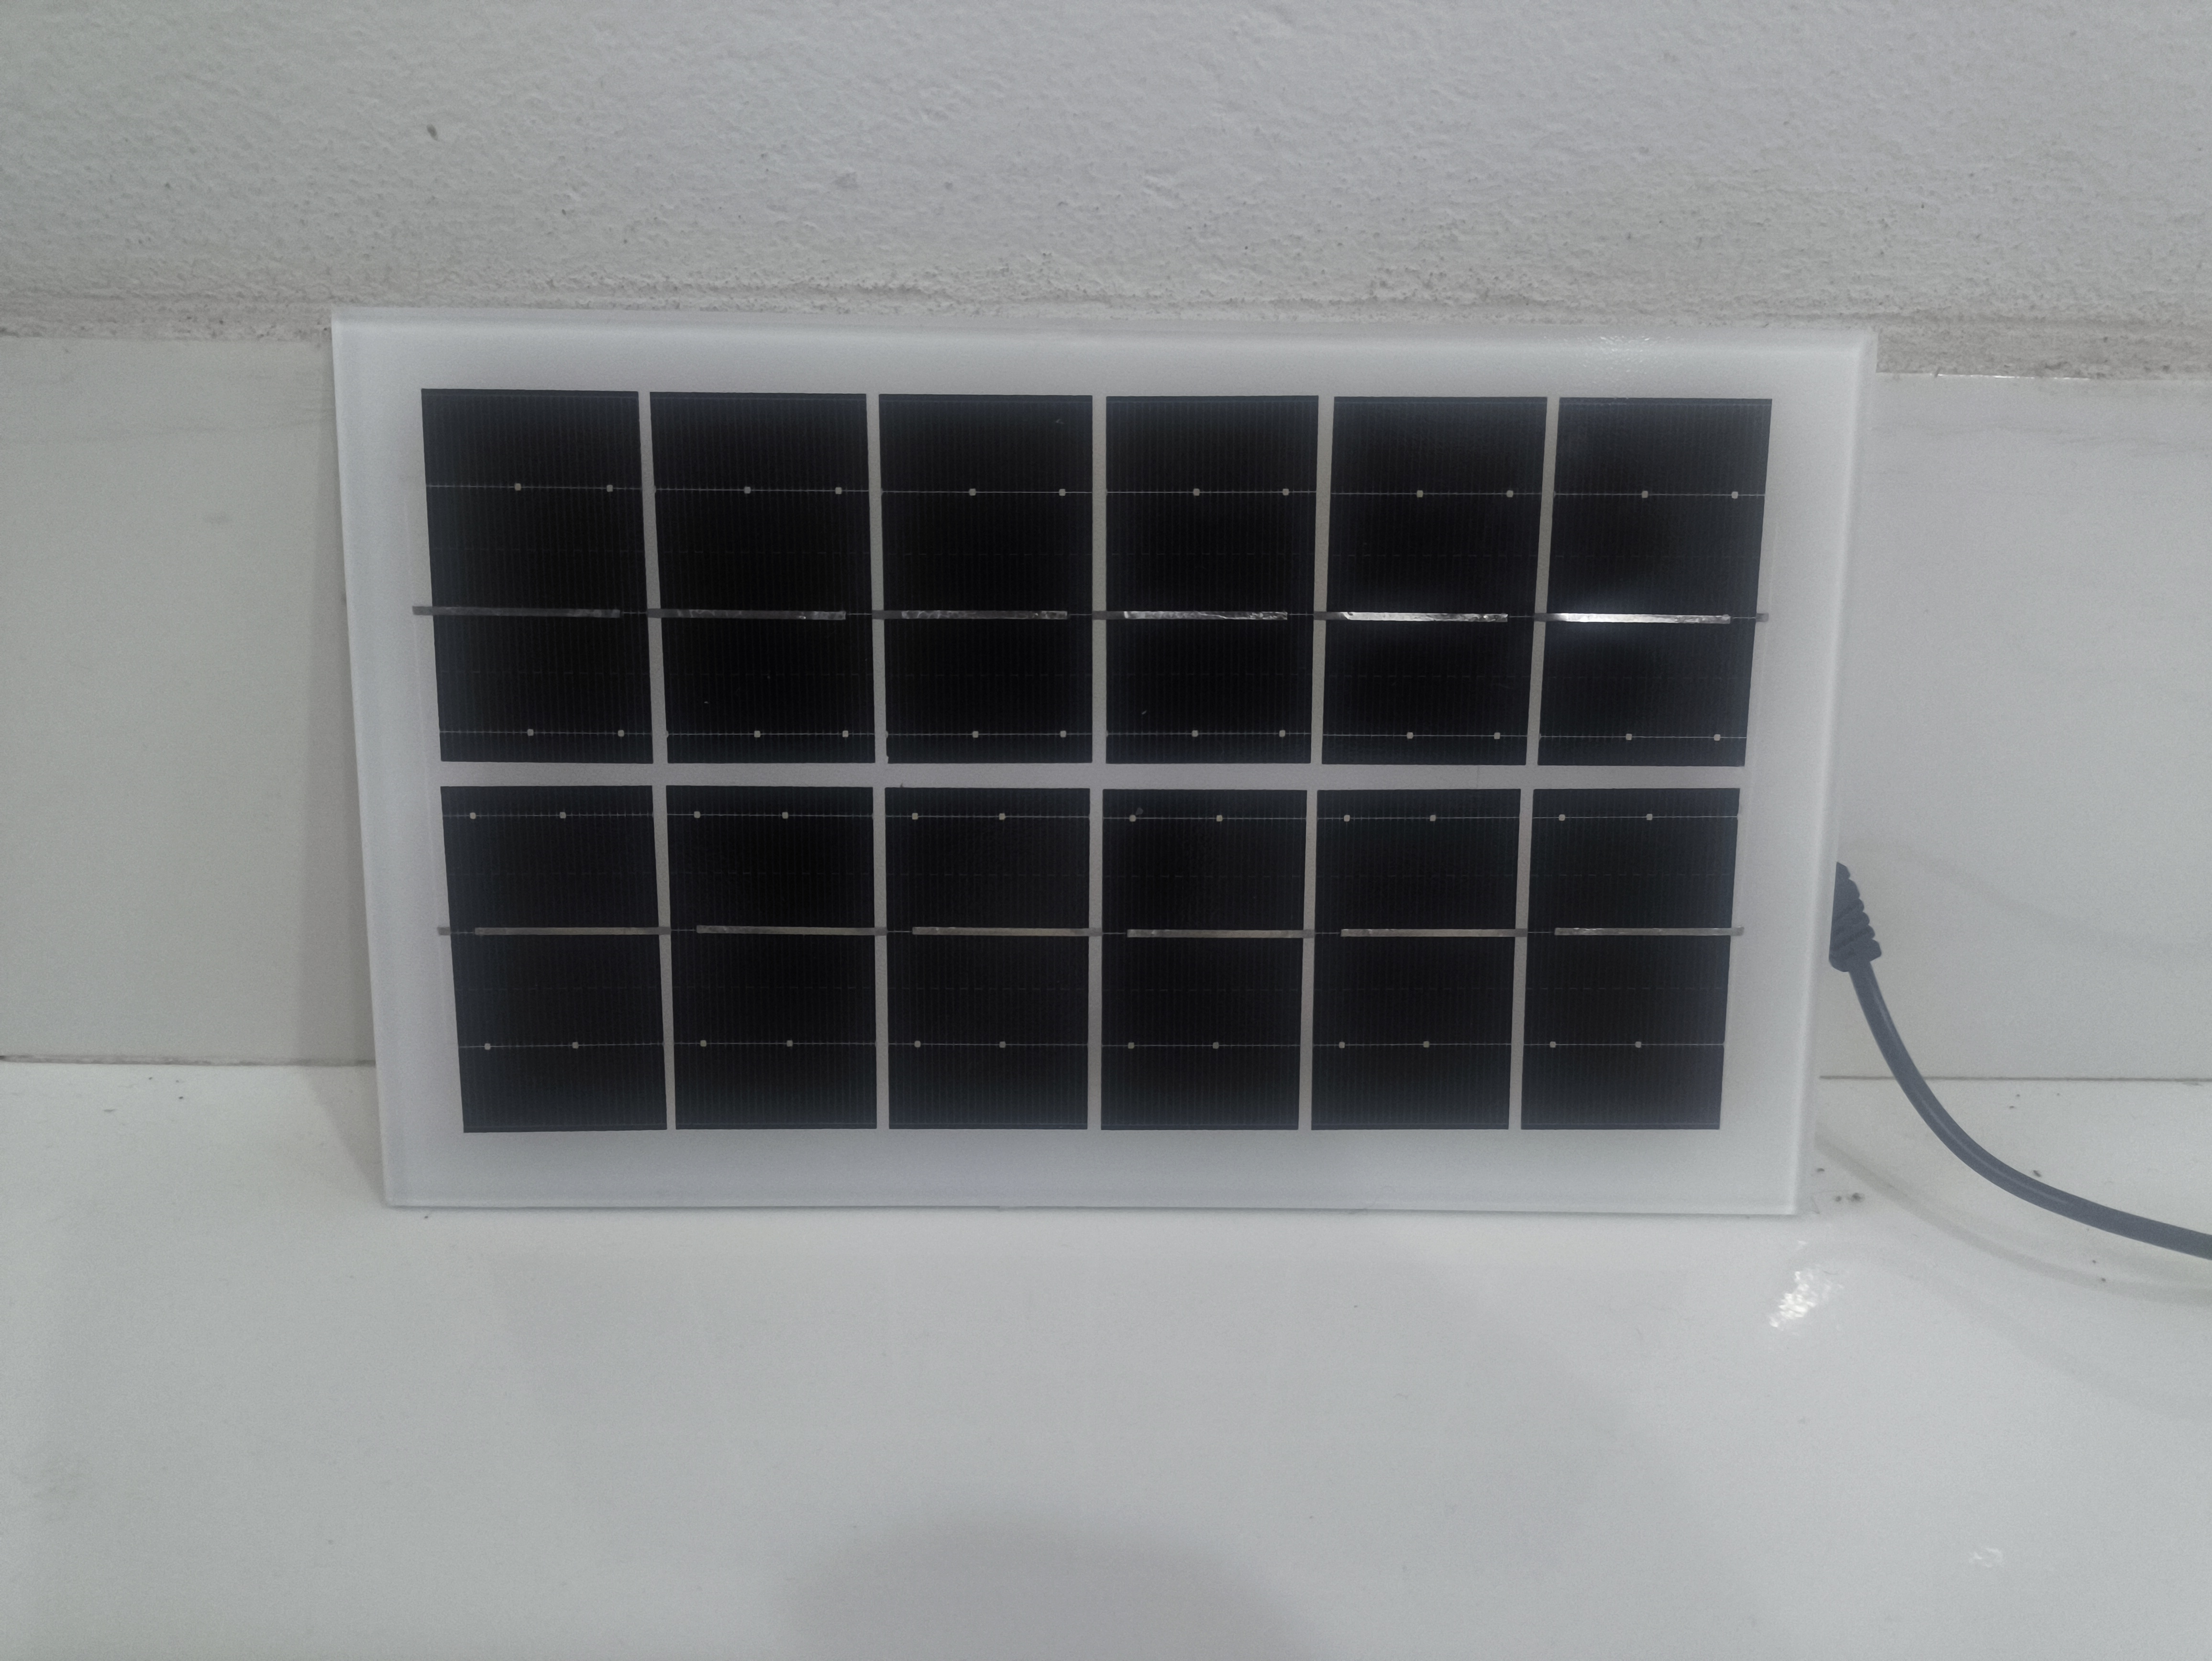
\includegraphics[width=0.7\textwidth]{Figuras/placa_solar.jpg}
    \caption{Placa solar fotovoltaica utilizada no experimento}
    \caption*{Fonte: Autor (2026).}
    \label{fig:placa_solar}
\end{figure}

O painel fotovoltaico é o elemento responsável pela conversão da energia solar em energia elétrica, sendo utilizado neste trabalho como fonte de dados para a análise do desempenho do sistema. Embora apresente capacidade de geração reduzida, sua aplicação mostra-se adequada aos objetivos propostos, uma vez que permite avaliar, de forma comparativa, o ganho percentual de eficiência proporcionado pelo sistema automatizado em relação a um sistema de eixo fixo.

A geração de energia de um painel fotovoltaico depende diretamente das condições ambientais, como temperatura e irradiância solar. Os testes e a avaliação de desempenho desses módulos são realizados com base em condições padronizadas e controladas, podendo ocorrer variações significativas na geração de energia quando tais condições não são atendidas. Nesse contexto, destacam-se as Condições Padrão de Teste (\textit{Standard Test Conditions} — STC), utilizadas como referência para a avaliação do desempenho dos módulos. Nessas condições, considera-se uma irradiância de 1000 W/m², temperatura da célula de 25~°C e espectro solar padrão, cenário no qual o painel opera próximo à sua potência nominal \cite{iec2016}.

Considerando essas premissas, mesmo com a utilização de um módulo de baixa potência, é possível obter dados experimentais consistentes para a análise do comportamento do sistema, permitindo a validação da proposta e a quantificação dos ganhos energéticos proporcionados pela automação.

\subsection{Módulo Sensor de Corrente e Sensor de Tensão}

Para a aquisição de dados elétricos do sistema, foram utilizados sensores de corrente e de tensão, elementos fundamentais para o monitoramento e avaliação do desempenho do painel fotovoltaico, conforme apresentado na Figura \ref{fig:sensores}.

\begin{figure}[H]
    \centering

    \begin{minipage}{0.45\linewidth}
        \centering
        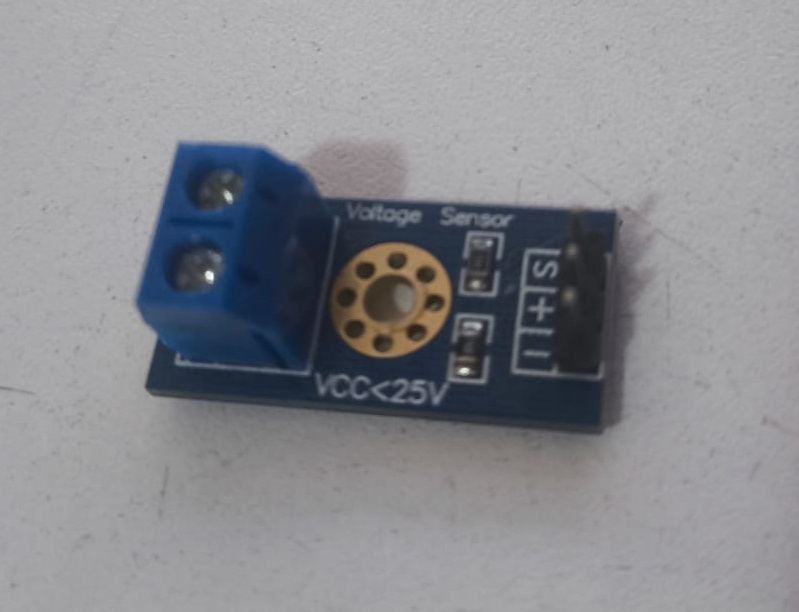
\includegraphics[height=5cm]{Figuras/sensor_tensao.jpeg}
        
        (a) Sensor de tensão
    \end{minipage}
    \hfill
    \begin{minipage}{0.45\linewidth}
        \centering
        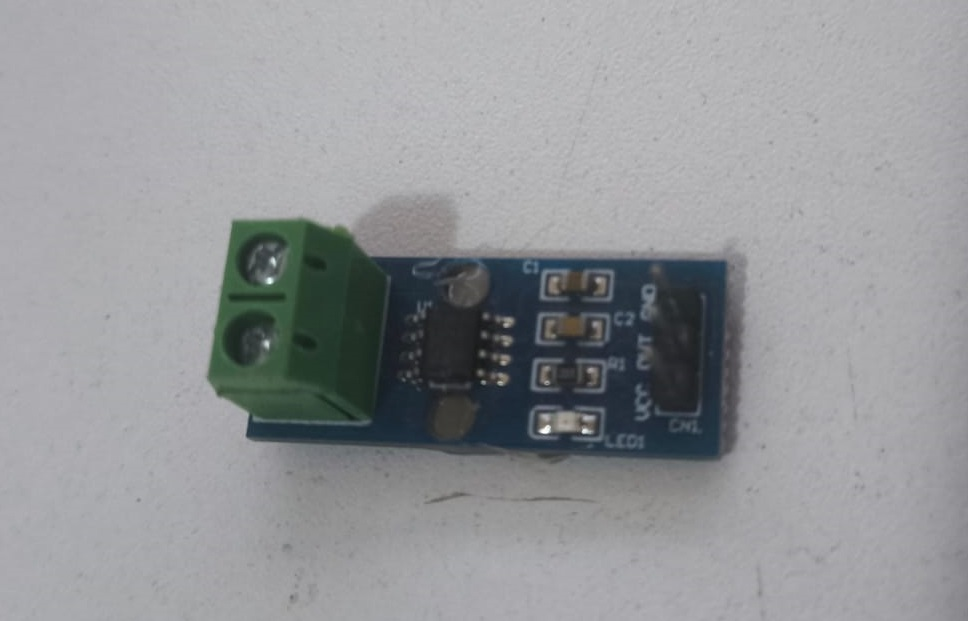
\includegraphics[height=5cm]{Figuras/sensor_corrente.jpeg}
        
        (b) Sensor de corrente
    \end{minipage}

    \caption{Sensores utilizados para aquisição de dados elétricos}
    \legend{Fonte: Autor (2026).}
    \label{fig:sensores}
\end{figure}


O sensor de corrente empregado foi o modelo ACS712, disponível em diferentes faixas de medição, como 5 A, 20 A e 30 A, sendo capaz de medir tanto corrente contínua quanto alternada. Esse dispositivo é baseado no efeito Hall, no qual a passagem de corrente elétrica por um condutor interno gera um campo magnético proporcional, detectado por um circuito integrado, permitindo a medição indireta da corrente elétrica \cite{allegro2019}.

O funcionamento do ACS712 baseia-se na conversão da corrente elétrica em um sinal de tensão analógico proporcional, geralmente centrado em torno de metade da tensão de alimentação do sensor. Essa característica permite ao microcontrolador interpretar tanto correntes positivas quanto negativas. Além disso, o sensor apresenta boa linearidade, isolamento elétrico entre o circuito de potência e o circuito de medição, bem como resposta rápida, o que o torna adequado para aplicações em sistemas embarcados e de monitoramento energético \cite{sparkfun_acs712}.

No contexto deste trabalho, o sensor de corrente é responsável por medir a intensidade da corrente gerada pelo painel fotovoltaico ao longo do dia, possibilitando a análise do comportamento do sistema sob diferentes condições de irradiância e posicionamento angular.

Complementarmente, foi utilizado um sensor de tensão baseado no princípio do divisor resistivo, com faixa de medição de até 25 V em corrente contínua. Esse módulo reduz a tensão de entrada para níveis compatíveis com as entradas analógicas do Arduino, garantindo a integridade do microcontrolador durante a aquisição dos dados \cite{usinainfo2024}.

A partir dos dados coletados pelos sensores de corrente e tensão, o sistema realiza o cálculo da potência elétrica instantânea gerada pelo painel fotovoltaico. Essa potência representa a taxa de conversão de energia elétrica em um determinado instante e é obtida conforme a relação fundamental entre essas grandezas:

\[
P = V \cdot I
\]

em que \(P\) representa a potência elétrica (em watts), \(V\) a tensão elétrica (em volts) e \(I\) a corrente elétrica (em amperes).

Essa relação indica que a potência gerada pelo sistema depende simultaneamente da tensão fornecida pelo painel e da corrente que circula no circuito. Dessa forma, variações nas condições ambientais, como irradiância e temperatura, influenciam diretamente essas grandezas. O sensor de tensão utilizado baseia-se no princípio do divisor de tensão resistivo, permitindo a redução de níveis de tensão mais elevados para valores compatíveis com a entrada analógica do microcontrolador \cite{sedra2016}. As medições obtidas permitem não apenas o cálculo da potência instantânea, mas também a análise do desempenho energético ao longo do tempo, sendo essenciais para a comparação entre o sistema automatizado e o sistema de eixo fixo.

Os sensores de corrente e tensão atuam, portanto, como dispositivos de aquisição de dados do sistema, permitindo a conversão de grandezas físicas em sinais elétricos interpretáveis pelo microcontrolador. Os dados obtidos são posteriormente processados, armazenados e utilizados na geração de indicadores de desempenho, evidenciando a integração entre hardware e software no desenvolvimento do sistema proposto e possibilitando a validação experimental dos resultados obtidos em simulação.

\subsection{Módulo Real Time Clock (RTC) DS1307}

Para a obtenção de informações temporais no sistema, foi utilizado o módulo \textit{Real Time Clock} (RTC), modelo DS1307, um dispositivo eletrônico dedicado à contagem contínua do tempo, capaz de manter seu funcionamento mesmo na ausência de alimentação principal, por meio de uma bateria auxiliar, conforme apresentado na Figura~\ref{fig:rtc}.

\begin{figure}[H]
    \centering
    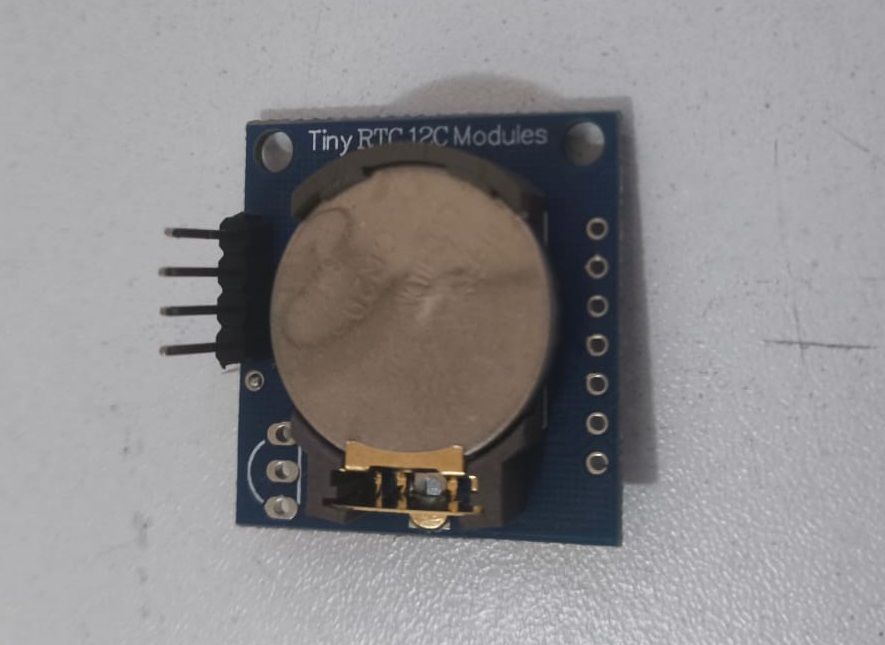
\includegraphics[width=0.6\textwidth]{Figuras/rtc.jpeg}
    \caption{Módulo RTC DS1307 utilizado no sistema}
    \caption*{Fonte: Autor (2026).}
    \label{fig:rtc}
\end{figure}

O DS1307 dispõe de um calendário completo, fornecendo dados de segundos, minutos, horas, dia da semana, data, mês e ano. A comunicação com o microcontrolador é realizada por meio do protocolo I2C (\textit{Inter-Integrated Circuit}), o que permite uma integração eficiente com plataformas embarcadas, como o Arduino, utilizando apenas duas linhas de comunicação (SDA e SCL) \cite{maxim2015}.

O dispositivo possui um circuito interno de detecção de falhas de energia (\textit{power-fail detect}), responsável pela comutação automática entre a alimentação principal e a bateria de backup, garantindo a continuidade da contagem do tempo e evitando a perda de dados temporais, o que o torna essencial em aplicações que exigem registro contínuo e confiável de informações \cite{maxim2015}.

Além disso, os dados fornecidos pelo RTC são fundamentais para o processo de aquisição e registro de dados experimentais. Cada leitura de tensão, corrente e potência é associada a um instante específico de tempo, permitindo a construção de séries temporais para análise do desempenho energético do sistema. Essa abordagem possibilita a comparação detalhada entre os sistemas, tanto em termos instantâneos quanto acumulados ao longo do dia.

Dessa forma, o módulo RTC DS1307 pode ser compreendido como um componente essencial para a organização temporal e sincronização dos dados, contribuindo diretamente para a confiabilidade das análises e para a validação experimental dos resultados obtidos.

\subsection{Módulo Leitor de Cartão Micro SD}

Para a gravação e armazenamento dos dados obtidos durante a execução do sistema, foi utilizado um módulo leitor de cartão microSD, responsável pela persistência das informações geradas ao longo do funcionamento do protótipo. Esse módulo permite o armazenamento dos dados em arquivos no formato texto, facilitando a posterior análise e visualização em softwares de planilhas eletrônicas, conforme apresentado na Figura~\ref{fig:sd}.

\begin{figure}[H]
    \centering
    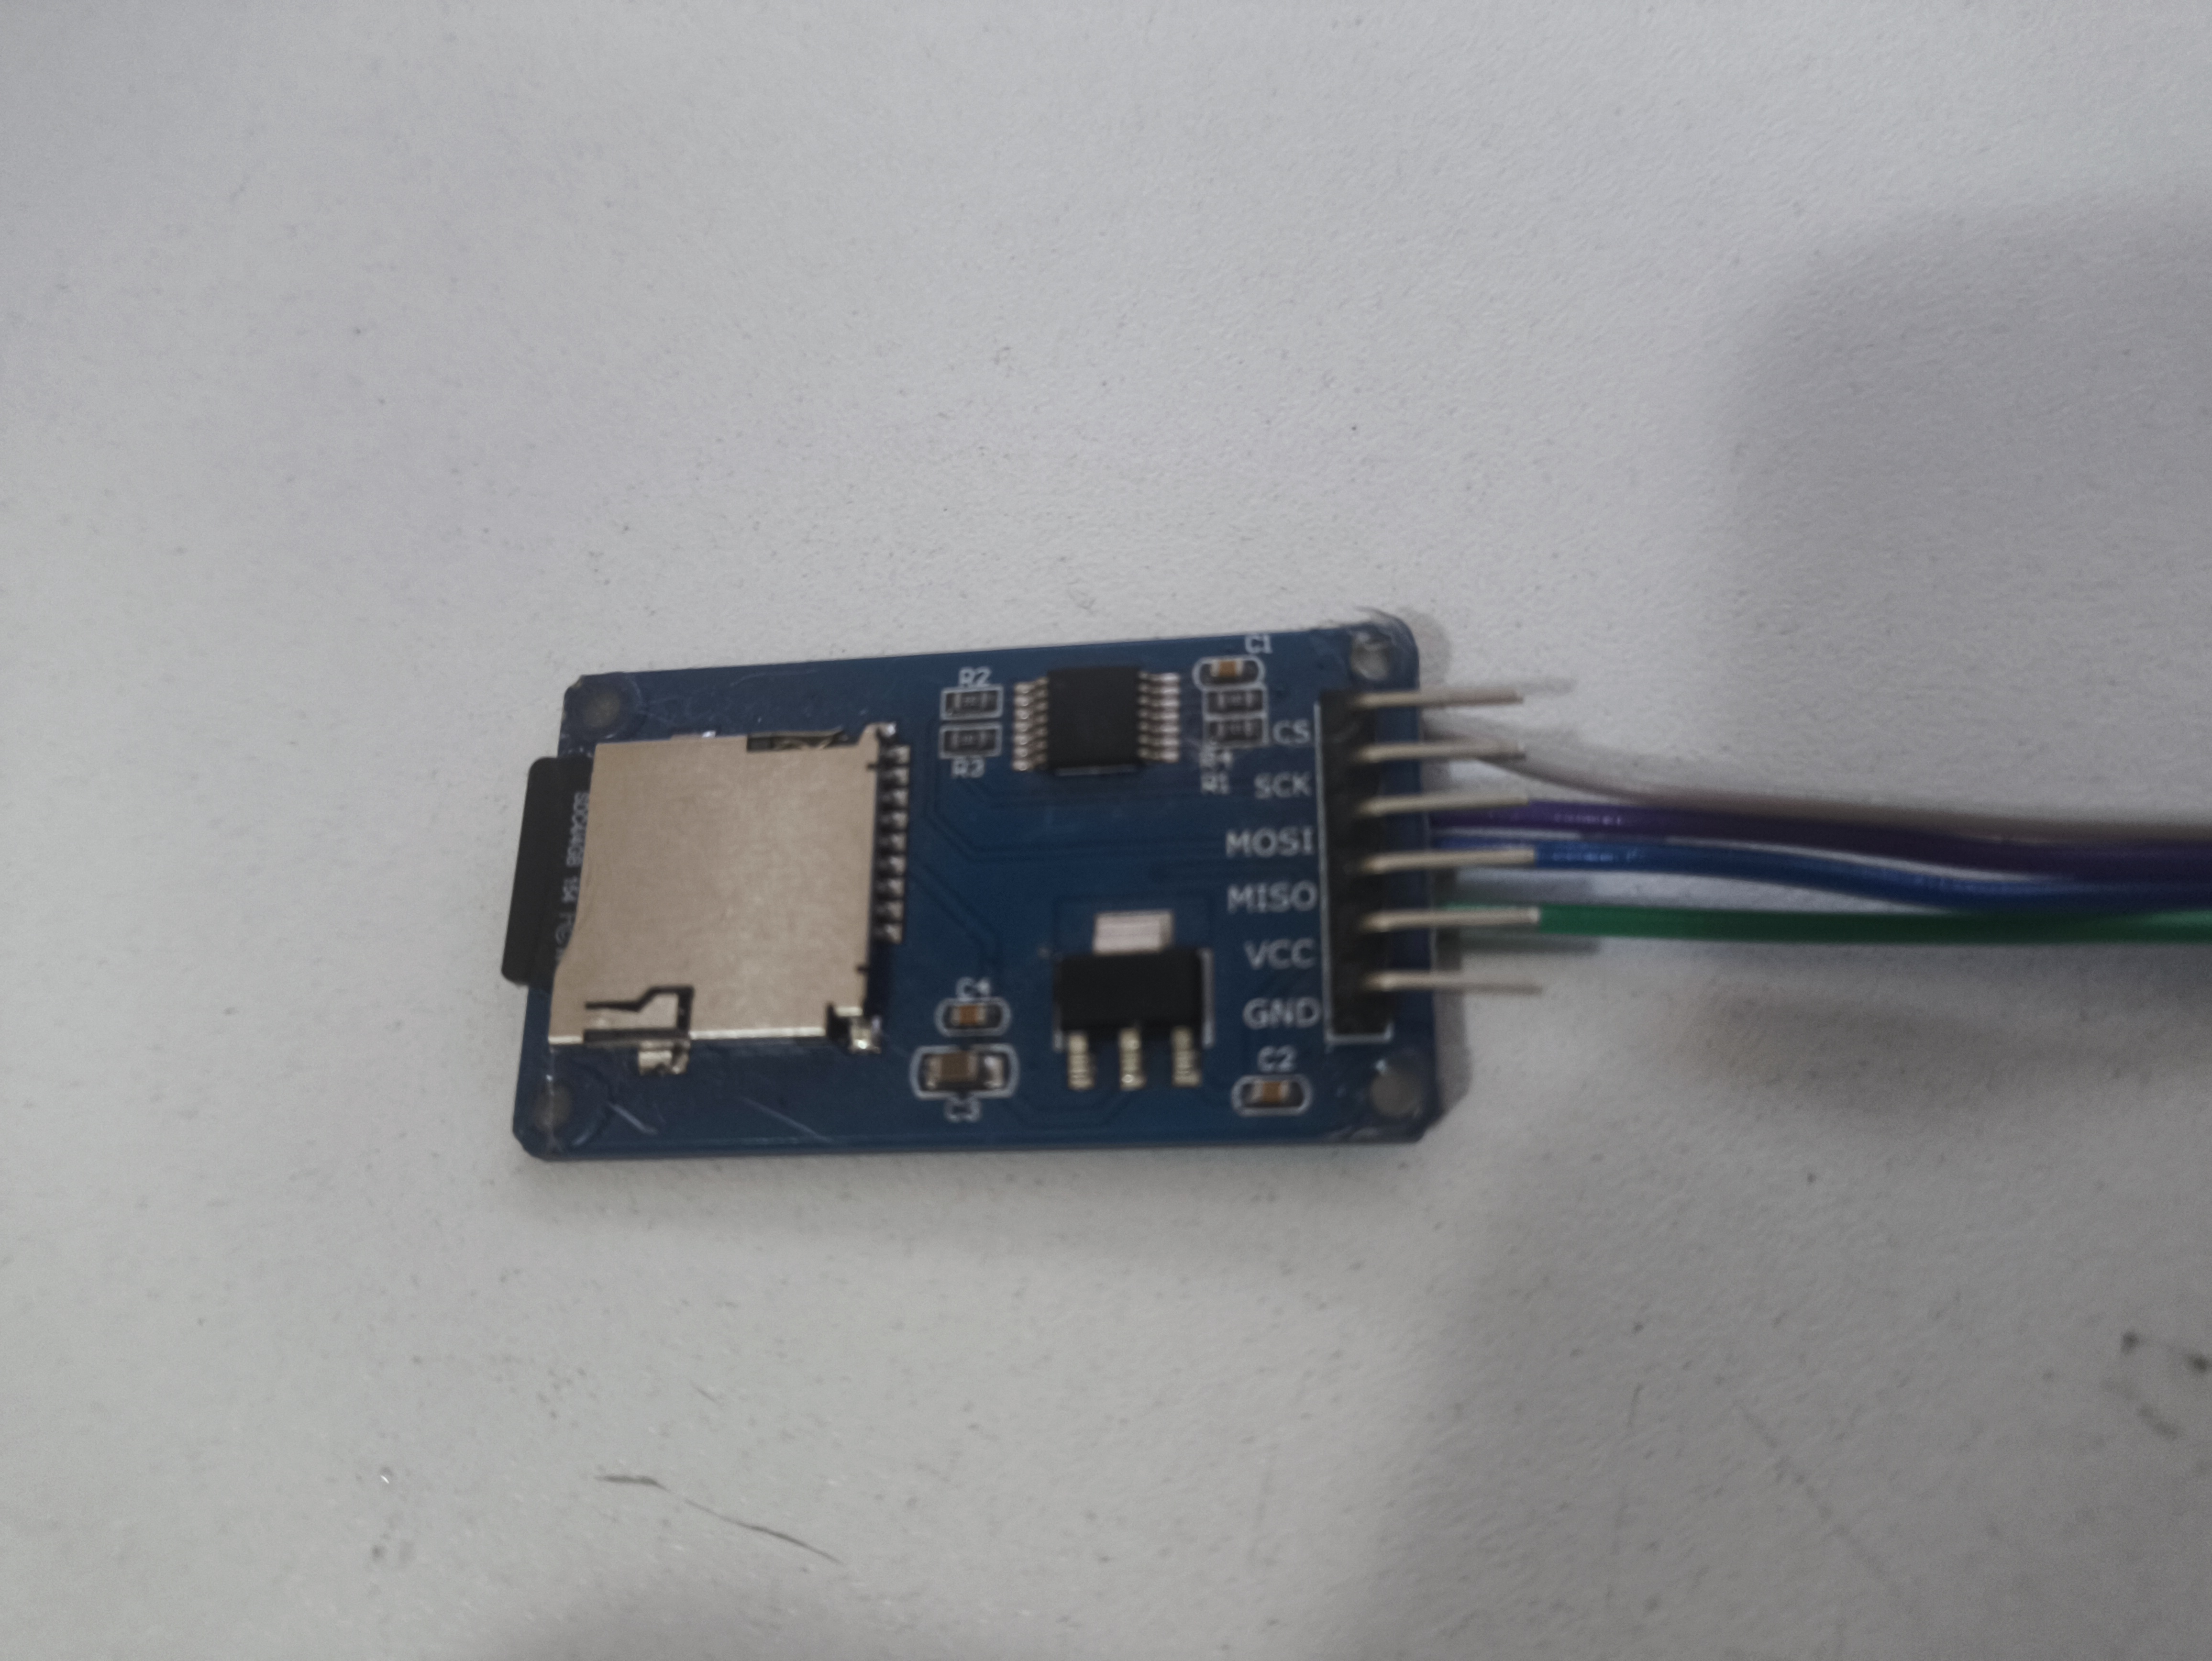
\includegraphics[width=0.6\textwidth]{Figuras/cartao_sd.jpg}
    \caption{Módulo leitor de cartão micro SD utilizado no sistema}
    \caption*{Fonte: Autor (2026).}
    \label{fig:sd}
\end{figure}

O módulo consiste em um dispositivo que integra um leitor de cartão microSD, permitindo a leitura e escrita de dados por meio de comunicação com o microcontrolador. Sua utilização é amplamente difundida em sistemas embarcados, especialmente em aplicações que demandam o registro contínuo de informações para análises posteriores, possibilitando o armazenamento organizado dos dados em arquivos digitais, como .txt ou .csv, o que facilita sua posterior análise em softwares de processamento de dados \cite{eletrogate2022}.

No contexto deste trabalho, o módulo é responsável pelo armazenamento estruturado dos dados coletados pelo sistema. Entre as variáveis registradas, destacam-se data, hora, tensão, corrente, potência elétrica e o ângulo de posicionamento do painel fotovoltaico. Esses dados são organizados em arquivos no cartão de memória, geralmente em formato texto (.txt) ou (.csv), o que facilita a posterior importação e análise em softwares como planilhas eletrônicas e ambientes de simulação.

Essa abordagem possibilita a construção de séries temporais detalhadas, fundamentais para a análise do comportamento energético do sistema. A partir desses dados, é possível calcular parâmetros como potência instantânea, energia acumulada e eficiência relativa, permitindo uma comparação consistente entre o sistema automatizado solar e o sistema de eixo fixo.

O módulo de cartão microSD desempenha, portanto, um papel essencial na etapa de persistência dos dados, assegurando a integridade,e a disponibilidade e a rastreabilidade das informações coletadas. Dessa forma, viabilizam-se análises quantitativas mais robustas e a validação experimental dos resultados obtidos.

\subsection{display de cristal líquido (Liquid Crystal Display – LCD)}

Para a visualização das informações do sistema, foi utilizado um display LCD 16x2 com interface I2C, que atua como meio de comunicação entre o sistema embarcado e o usuário. Esse tipo de display permite a exibição de caracteres alfanuméricos distribuídos em duas linhas de 16 colunas, sendo amplamente empregado em aplicações embarcadas devido à sua simplicidade, baixo custo e eficiência na apresentação de dados \cite{makerhero2022}, conforme apresentado na Figura~\ref{fig:lcd}.

\begin{figure}[H]
    \centering
    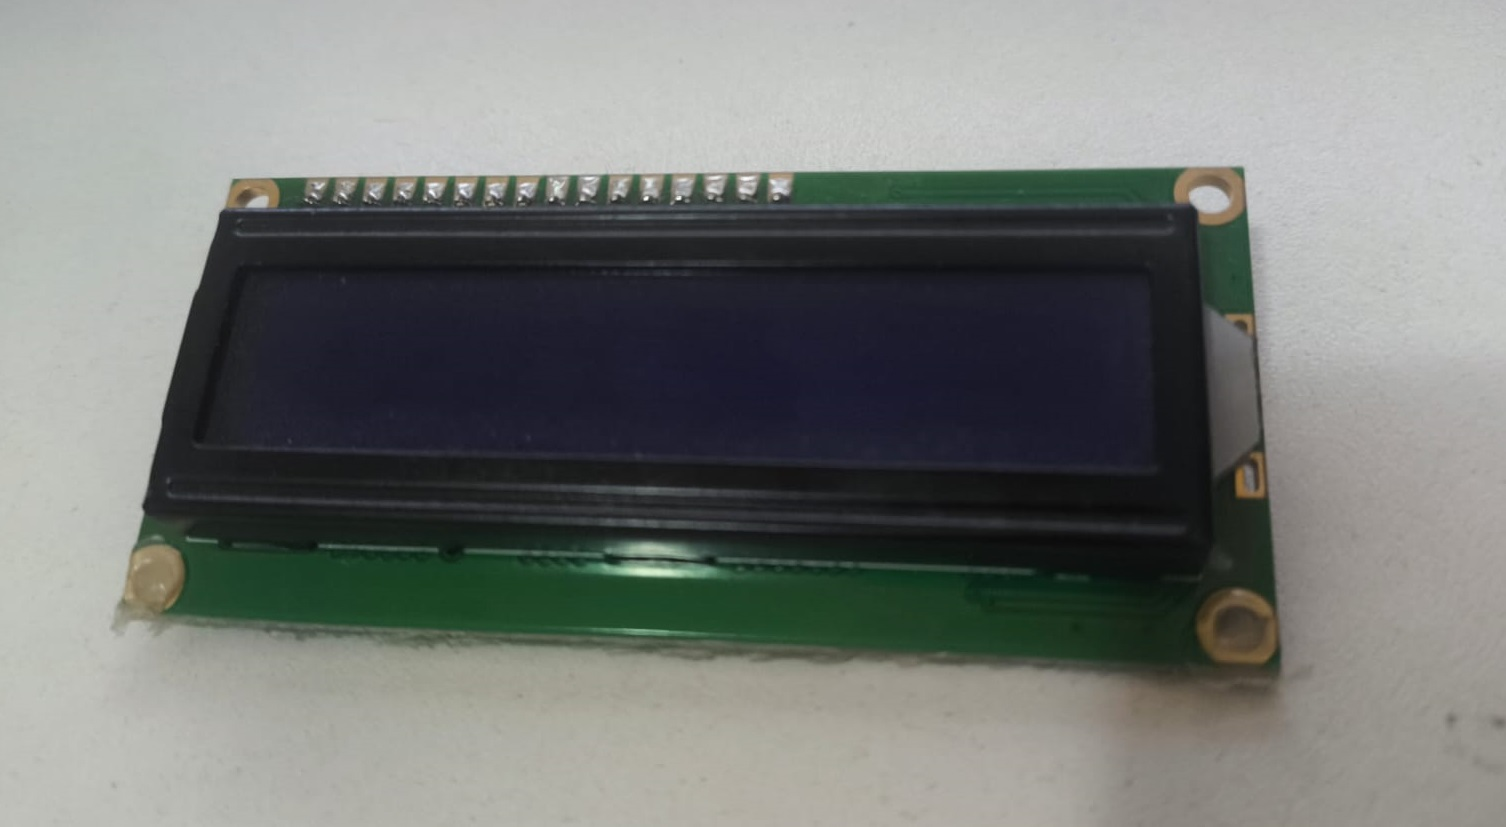
\includegraphics[width=0.6\textwidth]{Figuras/display.jpeg}
    \caption{Display LCD 16x2 com interface I2C utilizado no sistema}
    \caption*{Fonte: Autor (2026).}
    \label{fig:lcd}
\end{figure}


No contexto deste trabalho, o display LCD é utilizado para o monitoramento em tempo real do sistema automatizado, permitindo a visualização contínua das principais variáveis operacionais. Entre as informações exibidas, destacam-se a data e hora no formato DD/MM HH:MM, bem como as grandezas elétricas medidas, incluindo tensão (V), corrente (I), potência (P) e o ângulo de posicionamento do painel fotovoltaico (ANG).

Além da exibição dos dados de operação, o display também desempenha a função de indicar o estado do sistema, podendo apresentar mensagens de inicialização, funcionamento normal e possíveis condições de erro, como falhas na leitura de sensores ou na comunicação com módulos periféricos. Essa funcionalidade contribui para a validação prática do funcionamento do protótipo e auxilia na identificação de inconsistências durante os testes experimentais.

O display LCD 16x2 atua, portanto, como uma interface de saída fundamental no sistema, sendo responsável por apresentar, de forma clara, organizada e em tempo real, os dados processados pelo microcontrolador. Dessa forma, possibilita-se o acompanhamento contínuo das variáveis monitoradas, além de fornecer suporte à análise experimental e à verificação do desempenho do sistema desenvolvido.

\subsection{Programação do Sistema}

A programação do sistema foi desenvolvida utilizando o ambiente Arduino IDE (\textit{Integrated Development Environment}), disponibilizado gratuitamente pela plataforma Arduino. Esse ambiente permite a escrita, compilação e gravação de códigos no microcontrolador de forma simplificada, por meio da conexão da placa ao computador via interface USB. Após a seleção do modelo de placa e da porta de comunicação no ambiente, o código é transferido para o dispositivo, possibilitando sua execução embarcada \cite{arduinoIDE2026}. conforme apresentado na Figura \ref{fig:arduino_ide}.

\begin{figure}[H]
    \centering
    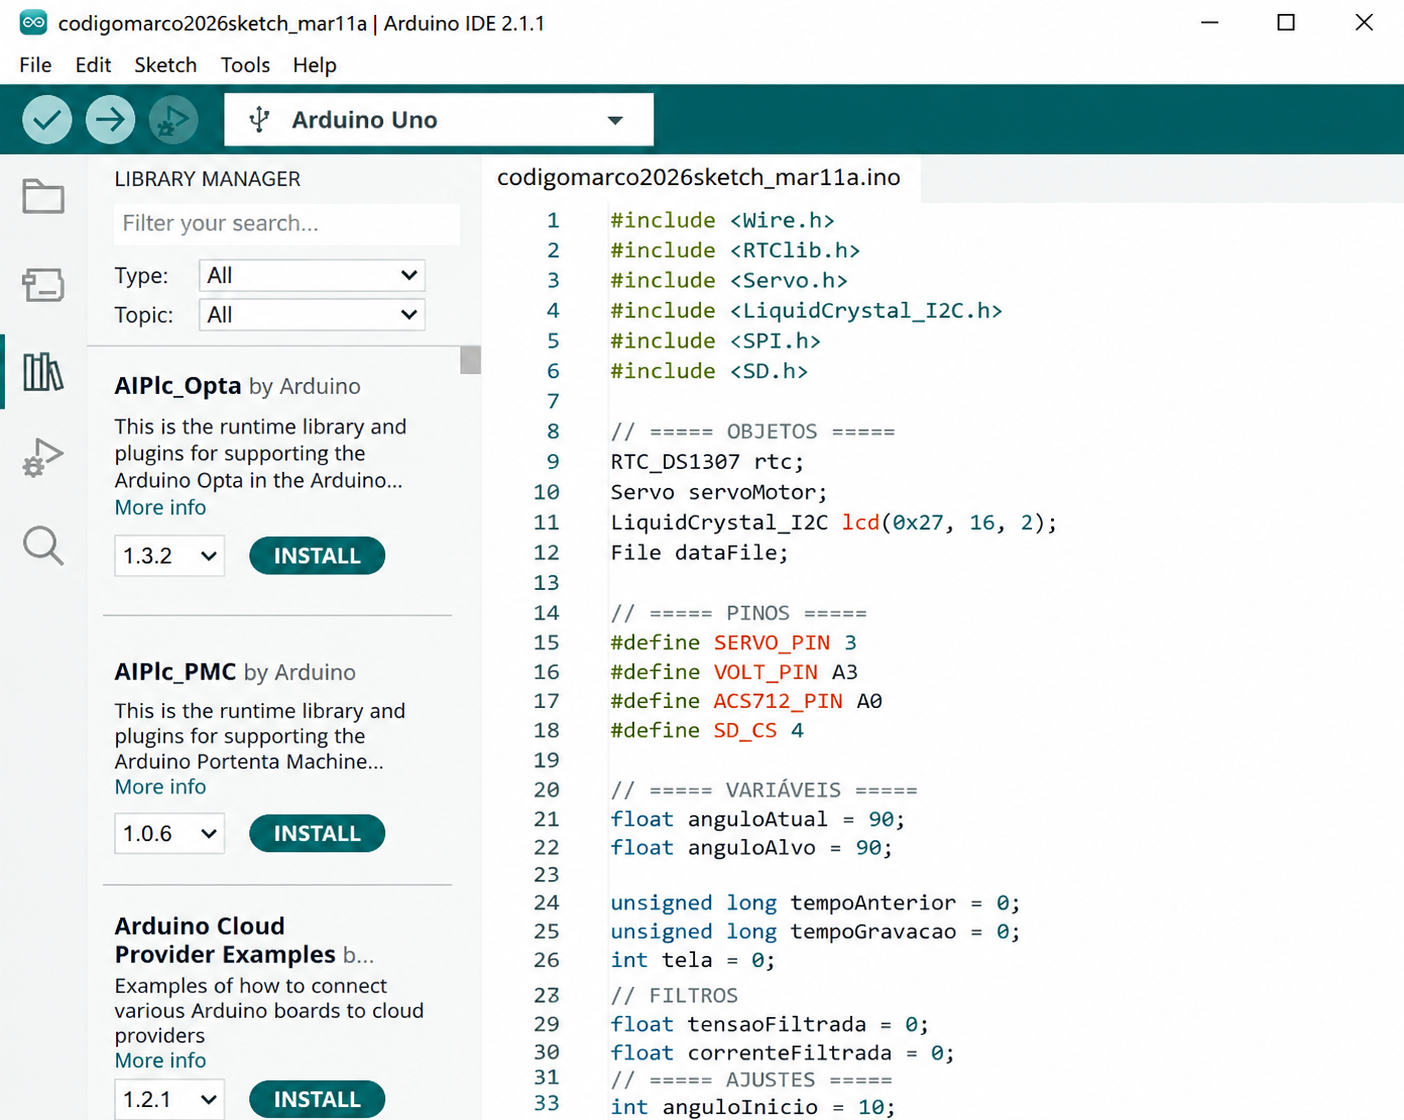
\includegraphics[width=1\textwidth]{Figuras/arduino_ide.png}
    \caption{Ambiente Arduino IDE com o código do sistema automatizado}
    \caption*{Fonte: Autor (2026).}
    \label{fig:arduino_ide}
\end{figure}

Os programas desenvolvidos nesse ambiente são denominados \textit{sketches} e são armazenados com a extensão .ino. Esses arquivos são estruturados, principalmente, em duas funções essenciais: \textit{setup()} e \textit{loop()}. A função \textit{setup()} é executada uma única vez e é responsável pela inicialização dos componentes e configurações do sistema, enquanto a função \textit{loop()} é executada continuamente, garantindo a operação cíclica do sistema ao longo do tempo \cite{arduinoSketch2026}.

Para viabilizar a comunicação com os dispositivos conectados, foram utilizadas bibliotecas específicas, responsáveis por abstrair detalhes de baixo nível e simplificar a implementação. Entre as principais, destacam-se bibliotecas para controle de servo motor, comunicação I2C (RTC e display LCD) e interface SPI (cartão microSD). O uso dessas bibliotecas contribui para a modularização do código, melhoria da legibilidade e redução da complexidade de desenvolvimento \cite{monk2017}.

No contexto deste trabalho, o software desenvolvido atua como núcleo de controle do sistema, sendo responsável por integrar todas as etapas de funcionamento. Inicialmente, o sistema realiza a leitura dos sensores de tensão e corrente por meio das entradas analógicas do microcontrolador, convertendo os sinais adquiridos em valores elétricos reais. A partir dessas grandezas, é efetuado o cálculo da potência instantânea gerada pelo painel fotovoltaico.

Paralelamente, o módulo RTC fornece as informações de data e hora, as quais são utilizadas como variáveis de entrada para o algoritmo de controle do posicionamento do painel. Com base nesses dados, o sistema determina o ângulo de inclinação adequado para cada instante do dia, enviando sinais de controle ao servo motor por meio de modulação por largura de pulso (PWM).

O software desenvolvido para o sistema automatizado foi implementado em plataforma Arduino e integra as funções de aquisição de dados, processamento, controle de posicionamento, otimização e armazenamento de informações. Seu funcionamento baseia-se inicialmente em um modelo de controle temporal, no qual são definidos parâmetros de referência correspondentes ao ângulo inicial do painel (início do dia), ao ângulo de referência para o meio-dia e ao ângulo final (fim do dia). A partir desses pontos, o sistema realiza uma interpolação do posicionamento ao longo do tempo, proporcionando um movimento suave e contínuo do painel fotovoltaico. Essa estratégia permite que, independentemente do horário em que o sistema seja inicializado, o painel seja automaticamente ajustado para a posição angular correspondente ao instante atual.

Além da automação baseado no horário, o sistema incorpora um algoritmo de otimização destinado a maximizar a geração de energia elétrica do módulo fotovoltaico. Para isso, é empregada uma abordagem empírica inspirada nas técnicas de rastreamento do ponto de máxima potência (\textit{Maximum Power Point Tracking} -- MPPT). Os métodos MPPT têm como objetivo maximizar a potência extraída dos módulos fotovoltaicos por meio do ajuste contínuo do ponto de operação do sistema \cite{Esram2007}. Neste trabalho, esse conceito foi adaptado ao posicionamento mecânico do painel solar, de modo que a busca pelo ponto de máxima potência ocorre por meio da variação do ângulo de posicionamento do módulo.

O algoritmo realiza uma varredura angular discreta em torno da posição estimada do painel, avaliando experimentalmente a potência gerada em cada posição. Com base nas medições obtidas, o sistema identifica o ângulo que proporciona a maior potência instantânea e ajusta o painel para essa condição. Dessa forma, o sistema não se limita apenas ao posicionamento calculado em função do horário, mas também considera o desempenho energético real do sistema, orientando o painel para a direção que resulta na máxima geração de energia disponível naquele instante.

Essa estratégia caracteriza uma adaptação dos princípios dos algoritmos MPPT para o domínio mecânico do sistema, permitindo que responda não apenas à posição teórica do Sol, mas também às condições reais de operação, como variações de irradiância, nebulosidade e pequenas imprecisões de alinhamento.

A estratégia adotada caracteriza-se como uma busca local baseada em dados reais obtidos pelos sensores instalados no sistema. Diferentemente dos métodos convencionais de automação que utilizam exclusivamente modelos astronômicos para determinar a posição do Sol, o algoritmo considera diretamente o desempenho energético do painel fotovoltaico, permitindo compensar fatores ambientais como nebulosidade, reflexões e pequenas imprecisões mecânicas.

Paralelamente às rotinas de controle e otimização, o sistema realiza a aquisição e o registro periódico de dados operacionais. As informações coletadas incluem data, hora, tensão, corrente, potência elétrica e ângulo de posicionamento do painel. Esses dados são armazenados em um cartão microSD, formando uma base de dados estruturada para análises posteriores. Simultaneamente, os valores são exibidos em tempo real em um display LCD, possibilitando o monitoramento imediato do desempenho do sistema durante sua operação.

Dessa forma, o software promove a integração entre as etapas de aquisição de dados, processamento, controle, otimização e armazenamento, evidenciando a aplicação prática de conceitos de sistemas embarcados, instrumentação eletrônica e automação. Essa integração é fundamental para a validação experimental do projeto, pois permite a comparação quantitativa entre o sistema fotovoltaico com automação e a configuração convencional de eixo fixo, possibilitando a avaliação dos ganhos energéticos obtidos pela estratégia proposta.


Por fim, destaca-se que o código-fonte completo desenvolvido neste trabalho encontra-se disponível no Apêndice A, permitindo a reprodução dos experimentos e a análise detalhada da implementação proposta.

\subsection{Sistema Eletrônico}

O sistema eletrônico do seguidor solar foi projetado com o objetivo de garantir confiabilidade operacional, estabilidade elétrica e eficiência na comunicação entre os módulos. O esquema geral é apresentado na Figura~\ref{fig:esquema}, na qual as conexões entre os componentes representam tanto o fluxo de energia quanto a troca de sinais de controle e dados.

\begin{figure}[H]
    \centering
    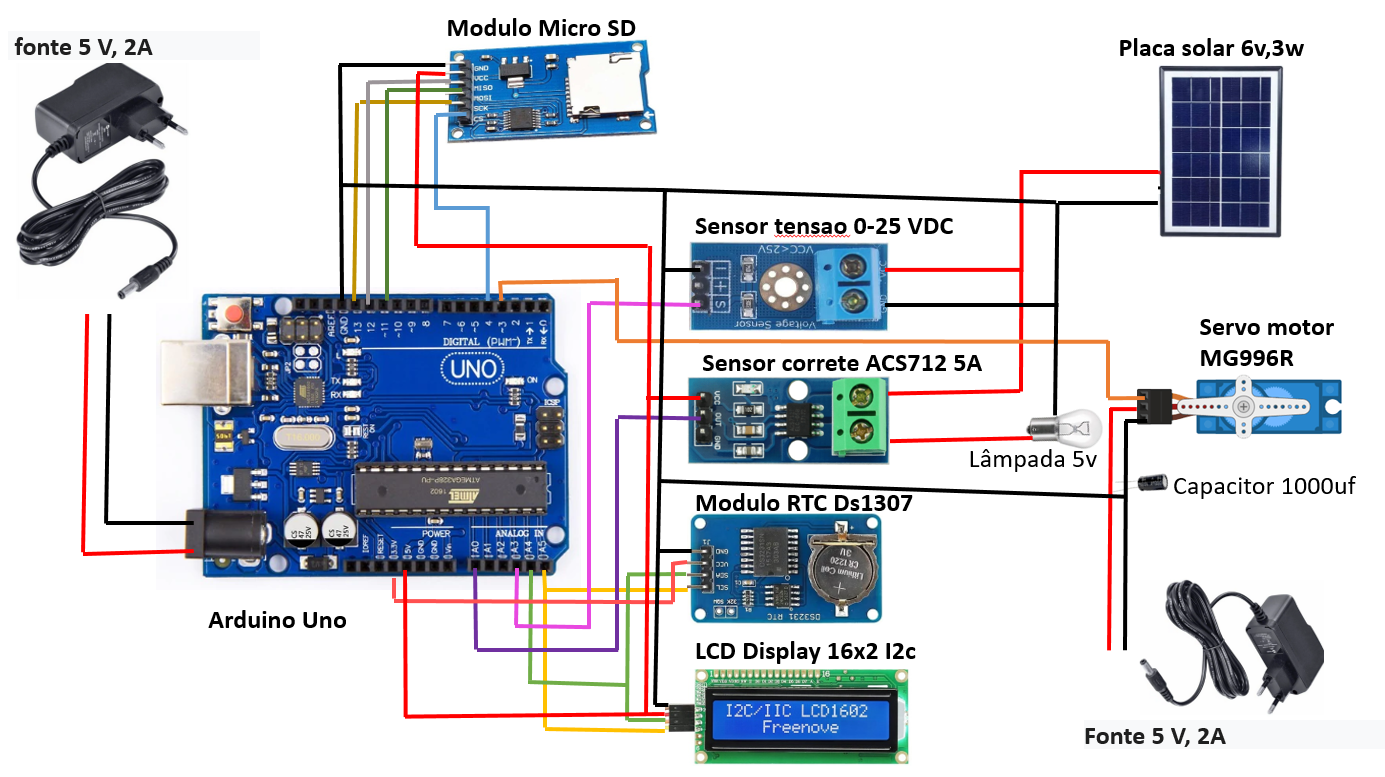
\includegraphics[width=0.9\textwidth]{Figuras/esquema.png}
    \caption{Esquema eletrônico do sistema automatizado}
    \caption*{Fonte: Autor (2026).}
    \label{fig:esquema}
\end{figure}

 Nesse contexto, o Arduino Uno atua como unidade central de controle, sendo alimentado por uma fonte externa de 5 V e 2 A conectada ao pino de alimentação apropriado da placa, o que garante o funcionamento do microcontrolador e dos periféricos a ele conectados, conferindo autonomia ao sistema.

O servo motor, responsável pela movimentação do painel fotovoltaico, possui alimentação independente de 5 V e 2 A, estratégia adotada para evitar sobrecarga no regulador de tensão do Arduino. O terminal positivo do servo é conectado à fonte externa de 5 V, enquanto o terminal negativo é ligado no polo negativo da fonte e paralelamente ao polo Ground (negativo do sistema - GND), o qual é comum a todos os componentes compartilhado com o Arduino. O sinal de controle é aplicado ao pino digital 3 da placa, que fornece um sinal PWM responsável pelo ajuste do ângulo de rotação. Adicionalmente, foi inserido um capacitor eletrolítico de 1000 µF / 16 V entre os terminais de alimentação do servo, com a finalidade de estabilizar a tensão e reduzir ruídos elétricos decorrentes da operação do motor.

O módulo RTC DS1307 é responsável pelo fornecimento de data e hora ao sistema. Sua alimentação é realizada pelo pino de 5 V do Arduino, com o terminal de terra conectado ao GND. A comunicação com o microcontrolador ocorre por meio do protocolo I2C, utilizando os pinos A5 (SCL) e A4 (SDA), o que permite a troca eficiente de dados temporais.

O módulo leitor de cartão microSD é alimentado pelo pino de 5 V do Arduino, com o terminal de terra conectado ao GND. A comunicação com o microcontrolador é realizada por meio do protocolo Serial Peripheral Interface (SPI), utilizando os pinos digitais 4 (CS), 13 (SCK), 12 (MISO) e 11 (MOSI), possibilitando a gravação e leitura de dados de forma confiável.

O display LCD 16x2 com interface I2C também é alimentado pelo pino de 5 V do Arduino, com conexão ao GND comum. Assim como o módulo RTC, utiliza o barramento I2C, compartilhando os pinos A5 (SCL) e A4 (SDA), o que reduz a quantidade de conexões físicas necessárias e simplifica a integração entre os dispositivos.

O sensor de corrente ACS712 é alimentado com 5 V e GND provenientes do Arduino, tendo seu pino de saída analógica conectado ao pino A0, permitindo a leitura da corrente elétrica por meio do conversor analógico-digital do microcontrolador. De forma análoga, o sensor de tensão possui sua saída conectada ao pino analógico A3, com o GND compartilhado com o restante do sistema, possibilitando a medição da tensão gerada pelo painel fotovoltaico.

As informações coletadas são organizadas na Tabela~\ref{tab:conexoes}, a qual apresenta as conexões entre os componentes do sistema e os respectivos pinos do Arduino. A estrutura é composta por duas colunas, sendo a primeira destinada à identificação dos componentes e a segunda à descrição de suas respectivas conexões elétricas e de comunicação.

\begin{table}[H]
\centering
\caption{Conexões entre os componentes do sistema}
\label{tab:conexoes}
\renewcommand{\arraystretch}{1.3}
\begin{tabular}{|p{4.5cm}|p{9cm}|}
\hline
\textbf{Componente} & \textbf{Conexões Arduino} \\
\hline

\textbf{Servo Motor (MG996R)} & 
Sinal → Pino 3 \newline
VCC → Fonte externa 5V \newline
GND → GND Arduino + Negativo Fonte \\
\hline

\textbf{RTC DS1307} & 
SDA → A4 \newline
SCL → A5 \newline
VCC → 5V \newline
GND → GND \\
\hline

\textbf{Display LCD 16x2 (I2C)} & 
SDA → A4 \newline
SCL → A5 \newline
VCC → 5V \newline
GND → GND \\
\hline

\textbf{Módulo Micro SD} & 
CS → Pino 4 \newline
SCK → Pino 13 \newline
MISO → Pino 12 \newline
MOSI → Pino 11 \newline
VCC → 5V \newline
GND → GND \\
\hline

\textbf{Sensor de Corrente (ACS712)} & 
OUT → A0 \newline
VCC → 5V \newline
GND → GND \\
\hline

\textbf{Sensor de Tensão} & 
OUT → A3 \newline
VCC → 5V \newline
GND → GND \\
\hline

\end{tabular}
\legend{Fonte: Autor (2026).}
\end{table}

Um aspecto fundamental do projeto é a utilização de um terra comum (GND) entre todos os componentes do sistema. Essa prática é essencial para garantir uma referência elétrica consistente, evitando erros de medição, ruídos e falhas de comunicação entre os dispositivos.

Para fins de validação experimental, foi implementado um segundo sistema fotovoltaico de referência, composto por um painel em posição fixa. Esse sistema foi desenvolvido de forma independente, com circuito próprio e aquisição de dados realizada em paralelo ao sistema automatizado. Os dados coletados por ambos os sistemas são armazenados separadamente, permitindo uma comparação direta e consistente entre as condições de operação.

A principal diferença entre os sistemas reside na presença do mecanismo de movimentação do painel solar, inexistente no sistema fixo. Dessa forma, torna-se possível avaliar quantitativamente o ganho de desempenho proporcionado pela automação do sistema, com base em parâmetros como potência instantânea, energia acumulada e eficiência relativa.

A adoção dessa abordagem experimental, baseada na operação de dois sistemas independentes sob condições equivalentes, aumenta a confiabilidade dos resultados obtidos, possibilitando a validação prática e a comparação consistente do desempenho do modelo proposto.

